
%%%%%%%%%% Practice Problems %%%%%

\practiceproblems
\noindent\problempart Put the following English arguments into standard form in logically structured English using variables for the terms. Be sure to include a translation key. Then identify mood and figure of the argument.
\begin{longtabu}{{X[1,l,p]X[9,l,p]}}
\textbf{Example}: &  No magical creatures are rainbow colored. Therefore, some unicorns are not rainbow colored, because all unicorns are magical creatures.
\end{longtabu}
\vspace{-22pt}
\begin{longtabu}{p{.05\linewidth}p{.45\linewidth}p{.3\linewidth}p{.1\linewidth}}

\textbf{Answer}: &
\vspace{-16pt}
\begin{description}
\item[$S$:] Unicorns
\item[$M$:] Magical Creatures
\item[$P$:] Things that are rainbow colored
\end{description}

&
\vspace{-16pt}
\begin{kormanize}
\premise{No $M$ are $P$.}
\premise{All $S$ are $M$.}
\vspace{-.5em}
\item [] \rule{0.5\linewidth}{.5pt}
\item[C:] Some $S$ are not $P$.}
\end{kormanize}

&
%\vspace{-16pt}
EAO-1

\end{longtabu}

\begin{exercises}

\item  Some beds are bunk beds, and all bunk beds are tall. So some beds are tall.

\answer{
\begin{longtabu}{X[2,l,p]X[2,l,p]X[1,l,p]}
\vspace{-16pt}
\begin{description}
\item[$S$:] Beds
\item[$M$:] Bunk beds.
\item[$P$:] Things that are tall
\end{description}

&
\vspace{-16pt}
\begin{kormanize*}
\item All $M$ are $P$
\item Some $S$ are $M$
\itemc Some $S$ are $P$
\end{kormanize*}

&

IAI-IV.

\end{longtabu}

}


\item No fluffy things are tusked pachyderms, but all tusked pachyderms are elephants. Therefore some elephants are not fluffy.

\answer{
\begin{longtabu}{X[2,l,p]X[2,l,p]X[1,l,p]}
\vspace{-16pt}
\begin{description}
\item[$S$:] Elephants
\item[$M$:]  Tusked pachyderms
\item[$P$:]  Things that are fluffy
\end{description}

&
\vspace{-16pt}
\begin{kormanize*}
\item  No $P$ are $M$
\item  All $M$ are $S$
\itemc Some $S$ are not $P$
\end{kormanize*}

&

EAO-4.
\end{longtabu}
}

\item Some strangers are not dangerous. After all, nothing that is dangerous is also a kitten. But some kittens are strangers.

\answer{
Notice this is conclusion-first.
\begin{longtabu}{X[2,l,p]X[2,l,p]X[1,l,p]}
\vspace{-16pt}
\begin{description}
\item[$S$:]  Strangers
\item[$M$:]  Kittens
\item[$P$:] Dangerous things
\end{description}

&
\vspace{-16pt}
\begin{kormanize*}
\item No $P$ are $M$
\item Some $M$ are $S$
\itemc Some $S$ are not $P$
\end{kormanize*}

&

EIO-4
\end{longtabu}
}
\item Some giant monsters are not things to be trifled with. This is because all kaiju are giant monsters and no kaiju is a creature to be trifled with.
\answer{
Notice that the major premise is given last here.

\begin{longtabu}{X[2,l,p]X[2,l,p]X[1,l,p]}
\vspace{-16pt}
\begin{description}
\item[$S$:]  Giant monsters
\item[$M$:]  Kaiju
\item[$P$:]  Things to be trifled with
\end{description}

&
\vspace{-16pt}
\begin{kormanize*}
\item  No $M$ are $P$
\item  All $M$ are $S$
\itemc Some $S$ are not $P$
\end{kormanize*}

&

EAO-3
\end{longtabu}
}

\item All parties are celebrations, because no celebrations are unhappy and no parties are unhappy.


\answer{
\begin{longtabu}{X[2,l,p]X[2,l,p]X[1,l,p]}
\vspace{-16pt}
\begin{description}
\item[$S$:]  Parties
\item[$M$:]  Unhappy things
\item[$P$:]  Celebrations
\end{description}

&
\vspace{-16pt}
\begin{kormanize*}
\item  No $P$ are $M$
\item  No $S$ are $M$
\itemc  All $S$ are $P$
\end{kormanize*}

&

EEA-2.
\end{longtabu}
}


\item Nothing that is deadly is safe. Therefore, some snakes are not deadly, because some snakes are safe.

\answer{
\begin{longtabu}{X[2,l,p]X[2,l,p]X[1,l,p]}
\vspace{-16pt}
\begin{description}
\item[$S$:]  Snakes
\item[$M$:]  Safe things.
\item[$P$:]  Deadly things
\end{description}

&
\vspace{-16pt}
\begin{kormanize*}
\item  No $P$ are $M$
\item  Some $S$ are $M$
\itemc  Some $S$ are not $P$
\end{kormanize*}

&

EIO-2.
\end{longtabu}
}

\item Godzilla is a character in a movie by the Toho company. This is because Godzilla is a kaiju, and some kaiju are Toho characters.

\answer{
\begin{longtabu}{X[3,l,p]X[2,l,p]X[1,l,p]}
\vspace{-16pt}
\begin{description}
\item[$S$:] Things identical to Godzilla
\item[$M$:]  Kaiju
\item[$P$:]  Toho characters
\end{description}

&
\vspace{-16pt}
\begin{kormanize*}
\item  Some $M$ are $P$
\item  All $S$ are $M$
\itemc All $S$ are $P$
\end{kormanize*}

&

IAA-1.
\end{longtabu}
}


\item No tyrannosaurs are birds. Therefore some pteranodons are not tyrannosaurs, because no pteranodons are birds.

\answer{
\begin{longtabu}{X[2,l,p]X[2,l,p]X[1,l,p]}
\vspace{-16pt}
\begin{description}
\item[$S$:]  Pteranodons
\item[$M$:]  Birds
\item[$P$:]  Tyrannosaurs
\end{description}

&
\vspace{-16pt}
\begin{kormanize*}
\item No $P$ are $M$
\item  No $S$ are $M$
\itemc Some $S$ are not $P$
\end{kormanize*}

&

EEO-2
\end{longtabu}
}

\item Every carnivorous animal is a college professor. Therefore all logicians are carnivores, because some college professors are not logicians.


\answer{
\begin{longtabu}{X[2,l,p]X[2,l,p]X[1,l,p]}
\vspace{-16pt}
\begin{description}
\item[$S$:] Logicians
\item[$M$:] College professors
\item[$P$:]  Carnivores
\end{description}

&
\vspace{-16pt}
\begin{kormanize*}
\item  All $P$ are $M$
\item  Some $M$ are not $S$
\itemc All $S$ are $P$
\end{kormanize*}

&

AOA-4
\end{longtabu}
}
\item Some balderdash is chicanery. Therefore no hogwash is chicanery, because all hogwash is balderdash.


\answer{
\begin{longtabu}{X[2,l,p]X[2,l,p]X[1,l,p]}
\vspace{-16pt}
\begin{description}
\item[$S$:] Hogwash
\item[$M$:] Balderdash
\item[$P$:]  Chicanery
\end{description}

&
\vspace{-16pt}
\begin{kormanize*}
\item Some $M$ are $P$
\item All $S$ are $M$
\itemc No $S$ are $P$
\end{kormanize*}

&

IAE-1.
\end{longtabu}
}


\end{exercises}

\noindent\problempart Put the following English arguments into standard form in logically structured English using variables for the terms. Be sure to include a translation key. Then identify mood and figure of the argument.


\begin{exercises}

\item No chairs are tables. But all tables are furniture. So some furniture are not chairs.

% P$_1$:  No $P$ are $M$
% P$_2$: All $M$ are $S$
%C: Some $S$ are not $P$

% EAO-1V Valid


\item All dogs bark, and some things that bark are annoying. Therefore some dogs are annoying.

%P$_1$: Some things that bark are annoying things
%P$_2$: All dogs are things that bark
%C: Some dogs are annoying things
%IAI-I

\item Some superheroes are not arrogant. This is because anyone who is arrogant is unpopular. But no superheroes are unpopular.

%P$_1$: All arrogant people are people who are unpopular
%P$_2$: No superheros are people who are unpopular
%C: Some superheros are not arrogant
% AEO-II Valid


\item Some mornings are not free time. But no evenings are mornings. Therefore no evenings are free time.

%P$_1$: Some $M$ are not $P$
%P$_2$: No $S$ are $M$
%C: No $S$ are $P$
%OEE-I

\item All veterinarians are doctors. Therefore some veterinarians are well trained, because all doctors are well trained.

%Valid AAI-I

\item No books are valueless. Therefore some books are not nonsense, because all nonsense is valueless.

%No $S$ are $M$
%All $P$ are $M$
%Some $S$ are not $P$


 \item No battleships are brightly colored, because no brightly colored things are lizards, and no battleships are lizards.
%P$_1$: No $P$ are $M$
%P$_2$: No $S$ are $M$
%C: No battleships are brightly colored.
%EEE-II

\item No octagons are curvilinear, because all circles are curvilinear and some octagons are circles.

%P$_1$: All $M$ are $P$
%P$_2$: Some $S$ are $M$
%C: No $S$ are $P$
%AIE-III

   \item Some eggs do not come from chickens. You can tell, because no milk comes from chickens, but all eggs are milk.

%P$_1$: No $M$ are $P$
%P$_2$: All $S$ are $M$
%C: Some $S$ are not $P$
%EAO-1II

\item Some ichthyosaurs are not eoraptors. Therefore some ichthyosaurs are mixosauruses, because some eoraptors are not mixosauruses.

%P$_1$: All $M$ are $P$
%P$_2$: Some $S$ are not $M$
%C: Some $S$ are $P$
%AOI-III Invalid Conclusion Middle
\end{exercises}

\noindent\problempart Put the following English arguments into standard form in logically structured English using variables for the terms. Be sure to include a translation key. Then identify mood and figure of the argument. Problems in this section are a little trickier than problems in Part A and Part B.


\begin{exercises}
\item  All spiders make thread, and anything that makes thread makes webs.  So for sure, all spiders make webs.

\item  Some children are not afraid to explore. For no one afraid to explore suffers from abandonment issues, and some children don't suffer from abandonment issues.


%Solution
% C = Things that are children
% E = Things that are (people and are) afraid to explore
% S = Things that suffer from abandonment issues
%
% 1. No E are S.
% 2. Some C are not S.
%      --------------------
% 3. Some C are not E.

% \includegraphics*[width=2.10in, height=1.73in, keepaspectratio=false]{img/image16}
% Invalid

\item  Every professional baseball player is a professional athlete, and no professional athlete is poor. No professional baseball player, thus, is poor.


\item  No horse contracts scrapie. So, because some animals contracting scrapie lose weight, there are horses that do not lose weight.

% H = Things that are horses.
% S = Things that are (animals and) contract scrapie.
% L = Things that lose weight.
%
% 1. No H are S.
% 2. Some S are L.
%----------------
% 3. Some H are not L.

% \includegraphics*[width=2.10in, height=1.73in, keepaspectratio=false]{img/image17}

%invalid

\item  Since everyone in this room is enrolled in logic, and since everyone at the college is enrolled in logic, everyone in this room is attending the college.

\item   All arguments are attempts to convince, and some attempts to convince are denials of autonomy. Therefore, some arguments are denials of autonomy.

\item  No one who likes smoked eel is completely reliable. For, everyone who likes smoked eel is a person with odd characteristics, and no one with odd characteristics is completely reliable.

\item Breaking an addiction requires self-control, and nothing requiring self-control is easy. Thus, breaking an addiction is never easy.

\item Jack is an American soldier in Iraq, and some American soldiers in Iraq are unable to sleep much. Hence, Jack is unable to sleep much.

\item All smurfs are blue, and no smurfs are tall. Therefore some tall things are not blue.

%P$_1$: All $M$ are $P$
%P$_2$: No $M$ are $S$
%C: Some $S$ are not $P$
% AEO-III Invalid


\end{exercises}

 \noindent\problempart Put the following English arguments into standard form in logically structured English using variables for the terms. Be sure to include a translation key. Then identify mood and figure of the argument. Problems in this section are a little trickier than problems in Part A and Part B.


\begin{exercises}
\item All Old World monkeys are primates. Some Old World monkeys are baboons. Therefore some primates are baboons

% All $M$ are $P$
% Some $M$ are $S$
% Some $S$ are $P$.
% Datisi (AII-3)

\item All gardeners are schnarf. And all extraterrestrials are gardeners. Therefore all extraterrestrials are schnarf.

% Barbara (AAA-I)

\item No corn chips are potato chips, but all corn chips are snacks, so no snacks are potato chips.

%P$_1$: No $M$ are $P$
%P$_2$: All $M$ are $S$
%C: No $S$ are $P$
%EAE-III Invalid

\item Everything in the attic is old and musty. Moreover, some pieces of furniture are old and musty. So, necessarily, some pieces of furniture are in the attic.

%$S$: Things that are pieces of furniture \newline
%					$M$: Things that are old and musty \newline
%					$P$: Things that are in the attic \newline


\item Some offices are pleasant places to work. All friendly places to work are workplaces. Therefore some workplaces are offices.

% Some $P$ are $M$
% All $M$ are $S$.
% Therefore some $S$ are $P$.
%Dimatis (IAI-IV)

% S: Supertaxon
% M: Taxon
% P: Overlapping taxon

\item Some rabbits are not white, but some snowdrifts are white. Therefore some snowdrifts are not rabbits.

%P$_1$: Some $P$ are not $M$
%P$_2$: Some $S$ are $M$
%C: Some $S$ are not $P$
%OIO-II Invalid Conclusion Middle

\item No airplanes are submarines, and some submarines are u-boats, so some airplanes are not u-boats.

%No $P$ are $M$ and some $M$ are $S$, so some $S$ are not $P$.
% No $P$ are $M$
% Some $M$ are $S$
% So some $S$ are not $P$.
% S: Subtaxon of M.
% M: Disjoint taxon
% P: Taxon
%Fresison (EIO-IV)

\item All rules have exceptions, but no commands from God have exceptions. So no rules are commands from God.

% All $P$ are $M$
% No $S$ are $M$
% No $S$ are $P$.
% Camestres (AEE-II)

\item All spies are liars, and some liars are not platypuses. Therefore some platypuses are spies.

%P$_1$: All $P$ are $M$
%	 P$_2$: Some $M$ are not $S$
%	 C: Some $S$ are $P$
%AOI-IV Invalid

\item Some bacteria are not harmful, and some harmful things are lions. Therefore some bacteria are lions.
%
%P$_1$: Some $P$ are not $M$
%	 P$_2$: Some $M$ are $S$
%	 C: Some $S$ are $P$
%OII-IV Invalid

\end{exercises}

\noindent\problempart Given the mood and figure, write out the full syllogism, using the term variables $S$, $M$, and $P$.
\begin{longtabu}{p{.1\linewidth}p{.9\linewidth}}
\textbf{Example}: &IAA-2 \\
\textbf{Answer}: & P$_1$: Some $P$ are $M$. \newline
P$_2$: All $S$ are $M$.
\vskip -6pt
\rule{0.2\linewidth}{.5pt} \newline
C: All $S$ are $P$.
\end{longtabu}

\begin{exercises}
\begin{longtabu}{X[1]X[1]}
\item EEE-4
\answer{
\begin{kormanize*}
\item No $P$ are $M$
\item No $M$ are $S$
\itemc No $S$ are $P$
\end{kormanize*}
}

&

\item EIE-1
\answer{
\begin{kormanize*}
\item No $M$ are $P$
\item Some $S$ are $M$
\itemc No $S$ are $P$
\end{kormanize*}
}

\\[-15pt]

\item AII-1
\answer{
\begin{kormanize*}
\item All $M$ are $P$
\item Some $S$ are $M$
\itemc Some $S$ are $P$
\end{kormanize*}
}

&

\item IIA-4
\answer{
\begin{kormanize*}
\item Some $P$ are $M$
\item Some $M$ are $S$
\itemc All $S$ are $P$
\end{kormanize*}
}

\\[-15pt]

\item IOO-2
\answer{
\begin{kormanize*}
\item Some $P$ are $M$
\item Some $S$ are not $M$
\itemc Some $S$ are not $P$
\end{kormanize*}
}

&

\item OEI-4
\answer{
\begin{kormanize*}
\item Some $P$ are not $M$.
\item  No $M$ are $S$.
\itemc Some $S$ are $P$.
\end{kormanize*}
}

\\[-15pt]

\item IIO-2
\answer{
\begin{kormanize*}
\item Some $P$ are not $M$
\item Some $S$ are not $M$
\itemc Some $S$ are not $P$
\end{kormanize*}
}

&

\item OAI-1
\answer{
\begin{kormanize*}
\item Some $M$ are $P$
\item All $S$ are $M$.
\itemc Some $S$ are $P$
\end{kormanize*}
}

\\[-15pt]

\item AAA-2
\answer{
\begin{kormanize*}
\item All $P$ are $M$
\item All $S$ are $M$
\itemc All $S$ are $P$
\end{kormanize*}
}

&

\item IAA-3
\answer{
\begin{kormanize*}
\item Some $M$ are $P$
\item All $M$ are $S$
\itemc All $S$ are $P$
\end{kormanize*}
}

\end{longtabu}
\end{exercises}

\noindent\problempart Given the mood and figure, write out the full syllogism, using the term variables $S$, $M$, and $P$


\begin{exercises}
\begin{longtabu}{X[1]X[1]}
\item EIO-1

&

\item AAI-4

\\[-15pt]

\item IIO-4

  &

\item AEA-4

\\[-15pt]

\item AOE-3

&

\item IAO-4

\\[-15pt]

\item OAI-3

&

\item IOE-2

\\[-15pt]

\item IAE-2

  &

\item EAO-2

\\[-15pt]

\end{longtabu}
\end{exercises}



%%%%%%%%%	 Practice problems %%%%%%%%%%%

\practiceproblems
\label{venn_proofs}
\problempart Use Venn diagrams to determine whether the following Aristotelian syllogisms are valid. You can check your answers against Table \ref{tab:unconditionally_valid}.

\begin{longtabu}{X[1,l,p]X[9,l,p]}
\textbf{Example}: &All $P$ are $M$ and no $M$ are $S$. Therefore, no $S$ are $P$. \\
\textbf{Answer}: &Valid (Calemes, AEE-4) \\
&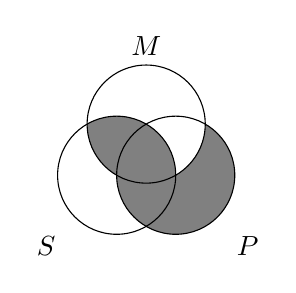
\begin{tikzpicture}
\def\firstcircle{(0,0) circle (.75cm)}
\def\secondcircle{(60:.75cm) circle (.75cm)}
\def\thirdcircle{(0:.75cm) circle (.75cm)}

	\begin{scope}[even odd rule] % Shade P without M
            \clip \secondcircle (-1,-1) rectangle (1.5,1.5);
        \fill[gray] \thirdcircle;
        \end{scope}

    \begin{scope} %shade overlap between S and M
      \clip \firstcircle;
      \fill[gray] \secondcircle;
    \end{scope}

\draw \firstcircle node[outer sep=.66cm, below left] {$S$};
\draw \secondcircle node [outer sep=.75cm, above] {$M$};
\draw \thirdcircle node [outer sep=.66cm, below right] {$P$};
\end{tikzpicture}\\
\end{longtabu}

\begin{exercises}

\item Some $P$ are not $M$, and no $M$ are $S$. Therefore, some $S$ are $P$.
\answer{\\
\begin{venns}
\shadeintersectred{\middlecircle}{\subjectcircle}
\drawsubsyl
\drawmidsyl
\drawpredsyl
\someexistthreefour
\end{venns}
\\
OEI-4 Invalid
}

\item All $M$ are $P$, and some $M$ are $S$. Therefore some $S$ are $P$.
\answer{\\
\begin{venns}
\shadecomplementred{\middlecircle}{\middlesquare}{\predicatecircle}
\drawsubsyl
\drawmidsyl
\drawpredsyl
\someexistseven
\end{venns}
\\
Datisi (AII-3) Valid
}

\item No $P$ are $M$, and some $S$ are $M$. Therefore, some $S$ are not $P$.
\answer{\\
\begin{venns}
\shadeintersectred{\predicatecircle}{\middlecircle}
\drawsubsyl
\drawmidsyl
\drawpredsyl
\someexistfive
\end{venns}
\\
Festino (EIO-2) Valid
}

\item No $M$ are $P$, and all $S$ are $M$. Therefore, no $S$ are $P$.
\answer{\\
\begin{venns}
\shadeintersectred{\middlecircle}{\predicatecircle}
\shadecomplementred{\subjectcircle}{\subjectsquare}{\middlecircle}
\drawsubsyl
\drawmidsyl
\drawpredsyl
\end{venns}
\\
Celarent (EAE-1) Valid
}
\item All $M$ are $P$, and no $M$ are $S$. Therefore, all $S$ are $P$.
\answer{\\
\begin{venns}
\shadecomplementred{\middlecircle}{\middlesquare}{\predicatecircle}
\shadeintersectred{\middlecircle}{\subjectcircle}
\drawsubsyl
\drawmidsyl
\drawpredsyl
\end{venns}
\\
AEA-3 Invalid
}
\item Some $M$ are not $P$, and some $M$ are $S$. Therefore, all $S$ are $P$.
\answer{\\
\begin{venns}
\drawsubsyl
\drawmidsyl
\drawpredsyl
\someexisttwofive
\someexistfiveseven
\end{venns}
\\

 OIA-3 Invalid
}

\item No $P$ are $M$, and some $S$ are not $M$. Therefore, some $S$ are not $P$.
\answer{\\
\begin{venns}
\shadeintersectred{\predicatecircle}{\middlecircle}
\drawsubsyl
\drawmidsyl
\drawpredsyl
\someexistonefour
\end{venns}
\\
EOO-2 Invalid
}

\item Some $P$ are $M$, and some $S$ are $M$. Therefore, no $S$ are $P$.
\answer{\\
\begin{venns}
\drawsubsyl
\drawmidsyl
\drawpredsyl
\someexistsixseven
\someexistfiveseven
\end{venns}
\\
IIE-2 Invalid
}

\item No $P$ are $M$, and all $S$ are $M$. Therefore no $S$ are $P$.
\answer{\\
\begin{venns}
\shadeintersectred{\predicatecircle}{\middlecircle}
\shadecomplementred{\subjectcircle}{\subjectsquare}{\middlecircle}
\drawsubsyl
\drawmidsyl
\drawpredsyl
\end{venns}
\\
Cesare (EAE-2) Valid
}
\item No $M$ are $P$ and all $S$ are $M$. Therefore some $S$ are not $P$
\answer{\\
\begin{venns}
\shadeintersectred{\predicatecircle}{\middlecircle}
\shadecomplementred{\subjectcircle}{\subjectsquare}{\middlecircle}

\drawsubsyl
\drawmidsyl
\drawpredsyl
\end{venns}
\\
EAO-1 Invalid \\
As we will learn in the next section, this argument would be valid if we added the premise ``Some $S$ exist.'' As a result, we will say this form is ``conditionally valid''
}
\end{exercises}

\noindent \problempart Use Venn diagrams to determine whether the following Aristotelian syllogisms are valid. You can check your answers against Table \ref{tab:unconditionally_valid}.

\begin{exercises}

\item No $M$ are $P$, and some $M$ are $S$. Therefore some $S$ are not $P$.
\answer{\\Ferison (EIO-III)}

\item Some $M$ are not $P$, and all $M$ are $S$. Therefore some $S$ are not $P$.
\answer{\\Bocardo (OAO-3)}

\item   No $M$ are $P$, and some $S$ are $M$. Therefore, some $S$ are not $P$.
 \answer{\\Ferio (EIO-I)}

\item All $M$ are $P$, and some $S$ are not $M$. Therefore, some $S$ are $P$.
\answer{\\AOI-I Invalid}

\item Some $P$ are $M$, and all $M$ are $S$. Therefore some $S$ are $P$.
 \answer{\\Dimatis (IAI-IV)}

\item Some $M$ are $P$, and all $S$ are $M$. Therefore, all $S$ are $P$.
\answer{\\IAA-I Invalid }

\item All $P$ are $M$, and all $M$ are $S$. Therefore, some $S$ are $P$.
\answer{\\AAI-IV Invalid }

 \item  All $P$ are $M$, and some $S$ are not $M$. Therefore, some $S$ are not $P$.
 \answer{\\Baroco (AOO-II)}

\item No $P$ are $M$, and all $M$ are $S$. Therefore no $S$ are $P$.
\answer{\\EAE-IV Invalid}

\item Some $P$ are $M$, and some $S$ are $M$. Therefore, some $S$ are $P$.
\answer{\\III-II Invalid}
 \end{exercises}

\noindent\problempart The arguments below are missing conclusions. Use Venn diagrams to determine what conclusion can be drawn from the two premises. If no conclusion can be drawn, write ``No conclusion.'' \label{no_conclusion_set1}

\begin{longtabu}{p{.15\linewidth}p{.85\linewidth}}
\textbf{Example 1}: & No $P$ are $M$ and some $M$ are not $S$. Therefore \underline{\hspace{2cm}} \\
\textbf{Answer}: & No conclusion\\
&

\begin{venns}
\shadeintersect{\predicatecircle}{\middlecircle}
\someexisttwo
\drawsubsyl
\drawmidsyl
\drawpredsyl
\end{venns}
\\
\textbf{Example 2}: & No $P$ are $M$ and  All $S$ are $M$. Therefore \underline{\hspace{2cm}} \\
\textbf{Answer}: &  No $S$ are $P$\\
&

\begin{venns}
\shadeintersect{\predicatecircle}{\middlecircle}
\shadecomplement{\subjectcircle}{\subjectsquare}{\middlecircle}
\drawsubsyl
\drawmidsyl
\drawpredsyl
\end{venns}

\end{longtabu}

\begin{exercises}

\item All $M$ are $P$, and all $S$ are $M$. Therefore \underline{\hspace{2cm}}.
\answer{ \hspace{-2.4cm} All $S$ are $P$. \\
\begin{venns}
\shadecomplementred{\middlecircle}{\middlesquare}{\predicatecircle}
\shadecomplementred{\subjectcircle}{\subjectsquare}{\middlecircle}
\drawsubsyl
\drawmidsyl
\drawpredsyl
\end{venns}
\\ Barbara (AAA-1)
}

\item All $M$ are $P$, and some $M$ are $S$. Therefore \underline{\hspace{2cm}}.
\answer{\hspace{-2.4cm} Some $S$ are $P$. \\
\begin{venns}
\shadecomplementred{\middlecircle}{\middlesquare}{\predicatecircle}
\drawsubsyl
\drawmidsyl
\drawpredsyl
\someexistseven
\end{venns}
\\Datisi (AII-3)
}

\item No $M$ are $P$ and some $S$ are not $M$. Therefore \underline{\hspace{2cm}}.
\answer{ \hspace{-2.4cm} No conclusion \\
\begin{venns}
\shadeintersectred{\middlecircle}{\predicatecircle}
\drawsubsyl
\drawmidsyl
\drawpredsyl
\someexistonefour
\end{venns}
 \\ EO?-1 Invalid
 }
\item Some $M$ are $P$, and some $S$ are $M$. Therefore \underline{\hspace{2cm}}.
\answer{ \hspace{-2.4cm} No conclusion \\
\begin{venns}
\drawsubsyl
\drawmidsyl
\drawpredsyl
\someexistsixseven
\someexistfiveseven
\end{venns}
\\  II?-1 Invalid
}
\item Some $P$ are $M$, and all $M$ are $S$. Therefore \underline{\hspace{2cm}}.
\answer{\hspace{-2.4cm} Some $S$ are $P$. \\
\begin{venns}
\shadecomplementred{\middlecircle}{\middlesquare}{\subjectcircle}
\drawsubsyl
\drawmidsyl
\drawpredsyl
\someexistseven
\end{venns}
\\ IAI-4 Valid (Dimatis)
 }
\item All $P$ are $M$ and no $M$ are $S$. Therefore \underline{\hspace{2cm}} .
\answer{\hspace{-2.4cm} No $S$ are $P$. \\
\begin{venns}
\shadecomplementred{\predicatecircle}{\predicatesquare}{\middlecircle}
\shadeintersectred{\subjectcircle}{\middlecircle}
\drawsubsyl
\drawmidsyl
\drawpredsyl
\end{venns}
\\Calemes (AEE-4)
}

\item No $M$ are $P$ and all $S$ are $M$. Therefore \underline{\hspace{2cm}} .
\answer{ \hspace{-2.4cm} No $S$ are $P$. \\
\begin{venns}
\shadeintersectred{\middlecircle}{\predicatecircle}
\shadecomplementred{\subjectcircle}{\subjectsquare}{\middlecircle}
\drawsubsyl
\drawmidsyl
\drawpredsyl
\end{venns}
\\ Celarent (EAE-1)
}

\item \label{itm:no_conclusion_set1_EEE} No $P$ are $M$, and no $M$ are $S$. Therefore \underline{\hspace{2cm}}.
\answer{\hspace{-2.4cm} No conclusion. \\
\begin{venns}
\shadeintersectred{\middlecircle}{\predicatecircle}
\shadeintersectred{\middlecircle}{\subjectcircle}
\drawsubsyl
\drawmidsyl
\drawpredsyl
\end{venns}
\\ EE?-4 Invalid
 }

\item No $M$ are $P$, and some $S$ are $M$. Therefore \underline{\hspace{2cm}}.
\answer{\hspace{-2.4cm} Some $S$ are not $P$. \\
\begin{venns}
\shadeintersectred{\middlecircle}{\predicatecircle}
\drawsubsyl
\drawmidsyl
\drawpredsyl
\someexistfive
\end{venns}
\\ Valid Ferio (EIO-1) .
}
\item Some $P$ are $M$, and some $S$ are $M$. Therefore \underline{\hspace{2cm}}.
\answer{\hspace{-2.4cm} No conclusion. \\
\begin{venns}
\drawsubsyl
\drawmidsyl
\drawpredsyl
\someexistsixseven
\someexistfiveseven
\end{venns}
 \\II?-2 Invalid
  }
  \end{exercises}

\noindent \problempart The arguments below are missing conclusions. Use Venn diagrams to determine what conclusion can be drawn from the two premises. If no conclusion can be drawn, write ``No conclusion.''

\begin{exercises}
\item Some $P$ are not $M$, and all $M$ are $S$. Therefore, \underline{\hspace{2cm}}.
 \answer{\\OAA-IV Invalid }

\item All $M$ are $P$, and some $S$ are $M$. Therefore \underline{\hspace{2cm}}.
\answer{\\Darii (AII-1) (unconditionally valid) }

\item All $P$ are $M$, and some $S$ are not $M$. Therefore \underline{\hspace{2cm}}.
\answer{\\Baroco (AOO-II) (unconditionally valid)}

\item Some $P$ are $M$, and all $M$ are $S$. Therefore \underline{\hspace{2cm}}.
\answer{\\Dimatis (IAI-IV) (unconditionally valid) }

\item All $P$ are $M$, and some $M$ are not $S$. Therefore \underline{\hspace{2cm}}.
\answer{\\AOA-IV Invalid}

\item No $M$ are $P$, and some $S$ are $M$. Therefore \underline{\hspace{2cm}}.
\answer{\\Ferio (EIO-I) (unconditionally valid)}

\item No $P$ are $M$, and no $S$ are $M$. Therefore \underline{\hspace{2cm}}.

\item Some $M$ are not $P$, and no $M$ are $S$. Therefore \underline{\hspace{2cm}}.

\item No $P$ are $M$, and all $S$ are $M$. Therefore \underline{\hspace{2cm}}.
\answer{\\EAA-II Invalid}

\item No $M$ are $P$, and some $M$ are $S$. Therefore \underline{\hspace{2cm}}.
\answer{\\Ferison (EIO-III) (unconditionally valid)}

\end{exercises}


\noindent\problempart
\label{ex_on_syllogism_patterns}
\answer{\\ The questions in this section were mostly meant to get you thinking about the issues we will be discussing in Section 5.4. Hopefully by looking for patterns in the 256 syllogisms, you can actually anticipate the rules we will demonstrate later on}

\begin{exercises}
\item Do you think there are any valid arguments in Aristotle's set of 256 syllogisms where both premises are particular? Why or why not? \label{itm:two_particulars}
\answer{\\No. You can intuitively see why this is the case when you remember that two particular premises could just be telling you about the existence of one or two particular objects, and you aren't going to be able to infer any generalities or any information about other particular objects from those two. For a more formal proof of why this is so, see see the discussion of Derived Rule 1 on page \ref{derived_rule_1}.}


\item Do you think there are any valid arguments in Aristotle's set of 256 syllogisms where both premises are negative? Why or why not?
\answer{\\No. You can see this by playing around with the Venn diagrams for negative statements, or by looking at the more formal proof of Rule 3 on page \ref{rule_3}.}

\item Can a valid argument have a negative statement in the conclusion, but only affirmative statements in the premises? Why or why not?
\answer{\\No. Again you can see this by playing around with Venn diagrams for negative statements, or by looking at the more formal proof of Rule 4 on page \ref{rule_4}}


\item Can a valid argument have an affirmative statement in the conclusion, but only one affirmative premise?
\answer{\\No, for the reasons stated above.}

\item Can a valid argument have two universal premises and a particular conclusion?
\answer{\\No, because the two universal statements do not have existential import, but the particular statement does. We will be talking more about this in the next section and in the proof of Rule 5 on page \ref{rule_5}.}
\end{exercises}


\practiceproblems
\noindent \problempart Use Venn diagrams to determine whether the following arguments are unconditionally valid, conditionally valid, or invalid. If they are conditionally valid, write out the premise you need to add. You can check your answers against Table \ref{tab:full_twentyfour}.

\begin{longtabu}{p{.1\linewidth}p{.9\linewidth}}
\textbf{Example}: & All $M$ are $P$ and all $M$ are $S$. Therefore some $S$ are $P$ \\
\textbf{Answer}: & Added premise: P$_3$: $M$ exists. \\
& \begin{center}
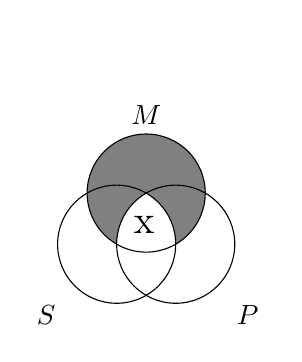
\begin{tikzpicture}
\def\firstcircle{(0,0) circle (.75cm)}
\def\secondcircle{(60:.75cm) circle (.75cm)}
\def\thirdcircle{(0:.75cm) circle (.75cm)}

\begin{scope}[even odd rule] % Shade M without P
\clip \thirdcircle (-1,-1) rectangle (2,2.75);
\fill[gray] \secondcircle;
\end{scope}


\begin{scope}[even odd rule] % Shade M without S
\clip \firstcircle (-1,-1) rectangle (2,2.75);
\fill[gray] \secondcircle;
\end{scope}


\draw \firstcircle node[outer sep=.66cm, below left] {$S$};
\draw \secondcircle node [outer sep=.75cm, above] {$M$};
\draw \thirdcircle node [outer sep=.66cm, below right] {$P$}
	node[xshift=-.4cm, yshift=.25cm](5){{\Large{x}}};
\end{tikzpicture}
\end{center}
\\ &
Conditionally valid (Darapti, AAI-3)
\end{longtabu}


\begin{exercises}

\item No $P$ are $M$, and all $S$ are $M$, so some $S$ are not $P$.
\answer{ \\
\begin{venns}

\shadeintersectred{\predicatecircle}{\middlecircle}
\shadecomplementred{\subjectcircle}{\subjectsquare}{\middlecircle}

\drawsubsyl
\drawmidsyl
\drawpredsyl

\end{venns}

Additional Premise: $S$ exists.

Cesaro (EAO-1I, conditionally valid)
\vspace{6pt}}

\item Some $P$ are $M$, and some $S$ are $M$. Therefore all $S$ are $P$.
\answer{ \\
\begin{venns}
\drawsubsyl
\drawmidsyl
\drawpredsyl
\someexistsixseven
\someexistfiveseven
\end{venns}

IIA-II Invalid
\vspace{6pt}}

\item No $M$ are $P$, and some $S$ are $M$. Therefore, some $S$ are not $P$.
\answer{ \\
\begin{venns}
\shadeintersectred{\middlecircle}{\predicatecircle}
\someexistfive
\drawsubsyl
\drawmidsyl
\drawpredsyl

\end{venns}

Ferio (EIO-I, unconditionally valid)
\vspace{6pt} }

\item  No $M$ are $P$, and all $S$ are $M$. Therefore, some $S$ are not $P$.
\answer{ \\
\begin{venns}
\shadeintersectred{\middlecircle}{\predicatecircle}
\shadecomplementred{\subjectcircle}{\subjectsquare}{\middlecircle}

\drawsubsyl
\drawmidsyl
\drawpredsyl

\end{venns}

Needed premise: Some $S$ exist.

Celaront (EAO-1, Conditionally valid)
\vspace{6pt} }

\item No $P$ are $M$, and some $M$ are $S$, so some $S$ are not $P$.
\answer{  \\
\begin{venns}

\shadeintersectred{\predicatecircle}{\middlecircle}

\drawsubsyl
\drawmidsyl
\drawpredsyl
\someexistfive

\end{venns}
\\Fresison (EIO-IV, unconditionally valid)
\vspace{6pt} }

\item All $P$ are $M$, and all $M$ are $S$, so some $S$ are $P$.
\answer{ \\
\begin{venns}
\shadecomplementred{\predicatecircle}{\predicatesquare}{\middlecircle}
\shadecomplementred{\middlecircle}{\middlesquare}{\subjectcircle}
\drawsubsyl
\drawmidsyl
\drawpredsyl
\end{venns}
\\Needed premise: $P$ exists. \\
Bamalip (AAI-IV, conditionally valid)
\vspace{6pt}  }

\item Some $P$ are not $M$, and some $M$ are $S$. Therefore all $S$ are $P$.
\answer{ \\
\begin{venns}

\drawsubsyl
\drawmidsyl
\drawpredsyl
\someexistthreefour
\someexistfiveseven
\end{venns}
\\ OIA-IV Invalid 7
 \vspace{6pt}}

\item No $P$ are $M$, and all $M$ are $S$. Therefore some $S$ are not $P$.
\answer{ \\
 \begin{venns}
\shadeintersectred{\predicatecircle}{\middlecircle}
\shadecomplementred{\middlecircle}{\middlesquare}{\subjectcircle}
\drawsubsyl
\drawmidsyl
\drawpredsyl
\end{venns}
\\Needed premise: $P$ exists. \\ Fesapo (AEO-IV, conditionally valid)
\vspace{6pt}}

\item All $M$ are $P$, and no $S$ are $M$. Therefore, some $S$ are $P$.
\answer{ \\
 \begin{venns}
\shadecomplementred{\middlecircle}{\middlesquare}{\predicatecircle}
\shadeintersectred{\middlecircle}{\subjectcircle}
\drawsubsyl
\drawmidsyl
\drawpredsyl
\end{venns}
\\ AEI-I Invalid
}
\item Some $M$ are $P$, and some $S$ are not $M$. Therefore, some $S$ are $P$.
\answer{ \\
\begin{venns}

\drawsubsyl
\drawmidsyl
\drawpredsyl
\someexistsixseven
\someexistonefour
\end{venns}
\\ IOI-I Invalid
}
\end{exercises}

\noindent \problempart Use Venn diagrams to determine whether the following arguments are unconditionally valid, conditionally valid, or invalid. If they are conditionally valid, write out the premise you need to add. You can check your answers against Table \ref{tab:full_twentyfour}.

\begin{exercises}

\item No $M$ are $P$, and all $M$ are $S$. Therefore some $S$ are not $P$.
\answer{Felapton (EAO-1II)  }

\item Some $M$ are $P$, and all $M$ are $S$. Therefore some $S$ are $P$.
\answer{Disamis (IAI-III) (unconditionally valid) }

\item All $M$ are $P$, and some $M$ are $S$, so no $S$ are $P$.
\answer{AIE-III Invalid }


\item No $M$ are $P$, and some $M$ are $S$, so some $S$ are not $P$.
\answer{Ferison (EIO-III) (unconditionally valid) }


\item Some $P$ are $M$, and some $S$ are not $M$, so no $S$ are $P$
\answer{IOE-II Invalid}

\item All $M$ are $P$, and all $S$ are $M$, so some $S$ are $P$.
\answer{Barbari (AAI-I) (conditionally valid) }

\item All $P$ are $M$, and no $M$ are $S$, so no $S$ are $P$.
\answer{Calemes (AEE-IV) (unconditionally valid) }

\item No $P$ are $M$, and all $S$ are $M$, so some $S$ are not $P$.
\answer{Camestros (EAO-1I) }

\item All $P$ are $M$, and no $M$ are $S$, so some $S$ are not $P$.
\answer{Calemos (AEO-IV) }

\item All $M$ are $P$, and some $S$ are $M$, so some $S$ are $P$.
\answer{Darii (AII-1) (unconditionally valid) }

\end{exercises}


%%%%%%%%% Practice Problems  %%%%%%%%%

\practiceproblems
\noindent \problempart Determine whether the following arguments are valid by seeing if they violate any of the five basic rules. If they are invalid, list the rules they violate. If they are valid, name their form. For conditionally valid arguments, label them valid if the existential premise is given explicitly, and invalid if it is not.

\begin{longtabu}{p{.15\linewidth}p{.9\linewidth}}
\textbf{Example 1}: &All $M$ are $P$, and all $S$ are $M$. Therefore no $S$ are $P$.\\
\textbf{Answer}: & Invalid. It violates rule 2, because $P$ is distributed in the conclusion but not the premises, and rule 4, because it has a negative conclusion and two affirmative premises.\\
\end{longtabu}

\begin{longtabu}{p{.15\linewidth}p{.9\linewidth}}
\textbf{Example 2}: & No $P$ are $M$, and all $S$ are $M$. Therefore some $S$ are not $P$.\\
\textbf{Answer}: & Invalid. It violates rule 5 because it is missing the existential premise ``Some $S$ exist.''\\
\end{longtabu}


\begin{exercises}

\item Some $M$ are $P$, and some $M$ are $S$. Therefore, no $S$ are $P$.

\answer{ It violates Rule 1 (middle term must be distributed), Rule 2 (terms distributed in the conclusion must be distributed in the premises), Rule 4 negative conclusion if and only if exactly one negative premise), and Derived Rule 1 (At least one universal premise.)}

\item Some $P$ are $M$, and some $M$ are not $S$. Therefore, all $S$ are $P$.

\answer{Invalid. It violates Rule 1 (middle term must be distributed), Rule 4 (negative conclusion if and only if exactly one negative premise) and Derived Rule 1 (At least one universal premise.)}

\item All $P$ are $M$, and no $M$ are $S$. Therefore, no $S$ are $P$.

\answer{ Valid. Calemes (AEE-4.)

\begin{venns}
\shadecomplementred{\predicatecircle}{\predicatesquare}{\middlecircle}
\shadeintersectred{\middlecircle}{\subjectcircle}
\drawsubsyl
\drawmidsyl
\drawpredsyl
\end{venns}
}

\item Some $P$ are not $M$, some $M$ are $S$. Therefore, all $S$ are $P$.

\answer{Invalid. It violates Rule 2 (terms distributed in the conclusion must be distributed in the premises) and Derived Rule 1 (At least one universal premise.)}


\item No $M$ are $P$, and all $S$ are $M$. Also, some $S$ exist. Therefore some $S$ are not $P$.

\answer{ Valid. Celeront (EAO-1). Notice that this does not violate rule 5 because the premise ``Some $S$ exist'' was included.

\begin{venns}
\shadeintersectred{\middlecircle}{\predicatecircle}
\shadecomplementred{\subjectcircle}{\subjectsquare}{\middlecircle}

\drawsubsyl
\drawmidsyl
\drawpredsyl
\end{venns}
}


\item All $P$ are $M$, and no $S$ are $M$. Therefore some $S$ are not $P$.

\answer{Invalid. This time we violate rule 5, because the existential premise was not included. If it were included, it would be Camestros (AEO-2)}

\item Some $M$ are $P$, and all $M$ are $S$. Therefore some $S$ are $P$.
\answer{Valid. Disamis (IAI-3)
\begin{venns}
\shadecomplementred{\middlecircle}{\middlesquare}{\subjectcircle}
\drawsubsyl
\drawmidsyl
\drawpredsyl
\someexistseven
\end{venns}
}

\item All $M$ are $P$, and all $S$ are $M$. Therefore some $S$ are not $P$.

\answer{Invalid. It violates Rule 2 (terms distributed in the conclusion must be distributed in the premises, Rule 4 (a negative conclusion requires exactly one negative premise), and Rule 5 (a particular conclusion must have at least one particular premise.)}

\item Some $M$ are not $P$, and all $S$ are $M$. Therefore, some $S$ are $P$.

\answer{Invalid. It violates Rule 1 (middle term must be distributed), and Rule 4 (a valid syllogism has a negative conclusion if and only if it has one negative premise.)}

\item Some $P$ are $M$, and some $M$ are not $S$. Therefore some $S$ are not $P$.

\answer{Invalid. It violates Rule 2 (terms distributed in the conclusion must be distributed in the premises) and Derived Rule 1 (No two particular premises) }

\end{exercises}

\noindent \problempart Determine whether the following arguments are valid by seeing if they violate any of the five basic rules. If they are invalid, list the rules they violate. If they are valid, name their form. For conditionally valid arguments, label them valid if the existential premise is given explicitly, and invalid if it is not.

\begin{exercises}

\item Some $M$ are not $P$, and no $S$ are $M$. Therefore, all $S$ are $P$.

\item No $M$ are $P$, and some $S$ are $M$. Therefore, some $S$ are not $P$.

\item All $P$ are $M$, and no $S$ are $M$. Therefore no $S$ are $P$.

\item All $P$ are $M$, and all $M$ are $S$. Also, some $S$ exist. Therefore some $S$ are $P$.

\item All $P$ are $M$, and no $S$ are $M$. Therefore some $S$ are not $P$.

\item All $M$ are $P$, and no $M$ are $S$. Therefore, some $S$ are $P$.

\item No $P$ are $M$, and all $M$ are $S$. Therefore, some $S$ are not $P$.

\item Some $M$ are not $P$, and some $M$ are $S$. Therefore, some $S$ are not $P$.

\item Some $M$ are $P$, and all $M$ are $S$. Therefore, some $S$ are not $P$.

\item No $P$ are $M$, and no $M$ are $S$. Therefore no $S$ are $P$.

\end{exercises}


\practiceproblems

\noindent\problempart Each of the following arguments are invalid. Prove that they are invalid by providing a counterexample that has the same form, but true premises and a false conclusion.

\begin{longtabu}{p{.1\linewidth}p{.9\linewidth}}
\textbf{Example}: & No pants are shirts, and no shirts are dresses, so some pants are not dresses. \\
\textbf{Answer}: & No dogs are reptiles, and no reptiles are mammals, so some dogs are not mammals.   \\
\end{longtabu}

%\begin{kormanize}
%\premise{No $P$ are $M$
%\premise{No $M$ are $S$
%\vspace{-.5em}
% \item [] \rule{0.6\linewidth}{.5pt}
%\item[C:] Some $S$ are not $P$
% \end{kormanize}
% EEO-IV Invalid Conclusion First
%



\begin{exercises}

\item Some mammals are animals, and some dogs are mammals. Therefore, all dogs are animals.

\answer{
\begin{longtabu}{X[1,l,p]X[1,l,p]}
\begin{kormanize}
\premise{Some $M$ are $P$
\premise{Some $S$ are $M$
\vspace{-.5em}
 \item [] \rule{0.6\linewidth}{.5pt}
\item[C:] All $S$ are $P$
 \end{kormanize}

&
\begin{kormanize*}
\item  Some mammals are chihuahuas
\item Some dogs are mammals
\itemc All dogs are chihuahuas
\end{kormanize*}
\end{longtabu}
}

\item Some evergreens are not spruces, and all spruces are trees. Therefore some trees are not evergreens.

\answer{
\begin{longtabu}{X[1,l,p]X[1,l,p]}

\begin{kormanize}
\premise{Some $P$ are not $M$
\premise{All $M$ are $S$
\vspace{-.5em}
 \item [] \rule{0.6\linewidth}{.5pt}
\item[C:] Some $S$ are not $P$
 \end{kormanize}
&
 \begin{kormanize*}
\item Some plants are not spruces
\item All spruces are trees.
\itemc Some trees are not plants.
\end{kormanize*}
\end{longtabu}
}

\item No wild animals are completely safe to be around, and some pigs are not completely safe to be around. Therefore some pigs are wild.
\answer{
\begin{longtabu}{X[1,l,p]X[2,l,p]}

\begin{kormanize}
\premise{No $P$ are $M$
\premise{Some $S$ are not $M$
\vspace{-.5em}
 \item [] \rule{0.6\linewidth}{.5pt}
\item[C:] Some $S$ are $P$
 \end{kormanize}
&
\begin{kormanize*}
\item No explosives are completely safe to be around
\item Some pigs are not completely safe to be around.
\itemc Some pigs are explosives.
\end{kormanize*}
\end{longtabu}
}

\item Some sodas are clear, and some healthy drinks are clear. Therefore no sodas are healthy.
\answer{
\begin{longtabu}{X[1,l,p]X[1,l,p]}
\begin{kormanize}
\premise{Some $P$ are $M$
\premise{Some $S$ are $M$
\vspace{-.5em}
 \item [] \rule{0.6\linewidth}{.5pt}
\item[C:] No $S$ are $P$
 \end{kormanize}
 &
\begin{kormanize*}
\item Some beverages are clear
\item Some healthy drinks are clear.
\itemc No beverages are healthy.
\end{kormanize*}
\end{longtabu}
}

\item No hamburgers are rocks, no igneous rocks are hamburgers. Therefore all igneous rocks are rocks.
\answer{
\begin{longtabu}{X[1,l,p]X[1,l,p]}

\begin{kormanize}
\premise{No $M$ are $P$
\premise{No $S$ are $M$
\vspace{-.5em}
 \item [] \rule{0.6\linewidth}{.5pt}
\item[C:] All $S$ are $P$
 \end{kormanize}
&
\begin{kormanize*}
\item No hamburgers are cats
\item No dogs are hamburgers.
\itemc All dogs are cats
\end{kormanize*}
\end{longtabu}
}

\item Some plants are not food, and some foods are vegetables. Therefore some plants are vegetables.
\answer{
\begin{longtabu}{X[1,l,p]X[1,l,p]}

\begin{kormanize}
\premise{Some $P$ are not $M$
\premise{Some $M$ are $S$
\vspace{-.5em}
 \item [] \rule{0.6\linewidth}{.5pt}
\item[C:] Some $S$ are $P$
 \end{kormanize}
&
\begin{kormanize*}
\item Some plants are not food
\item Some foods are animal products.
\itemc Some plants are animal products
\end{kormanize*}
\end{longtabu}
}
\item All apartment buildings are buildings, and some buildings are residential buildings. Therefore some residential buildings are not apartment buildings.
\answer{
\begin{longtabu}{X[1,l,p]X[1,l,p]}
\begin{kormanize}
\premise{All $P$ are $M$
\premise{Some $M$ are $S$
\vspace{-.5em}
 \item [] \rule{0.6\linewidth}{.5pt}
\item[C:] Some $S$ are not $P$
 \end{kormanize}
 &

\begin{kormanize*}
\item All dogs are mammals
\item  Some mammals are animals
\itemc Some dogs are not animals.
\end{kormanize*}

\end{longtabu}
}

\item No foods are games, and some games are video games. Therefore no video games are food.
\answer{
\begin{longtabu}{X[1,l,p]X[1,l,p]}

\begin{kormanize}
\premise{No $P$ are $M$
\premise{Some $M$ are $S$
\vspace{-.5em}
 \item [] \rule{0.6\linewidth}{.5pt}
\item[C:] No $S$ are $P$
 \end{kormanize}

&
\begin{kormanize*}
\item No mammals are reptiles
\item Some reptiles are pets
\itemc No pets are mammals
\end{kormanize*}
\end{longtabu}
}
\item Some trucks are rentals, and no cars are trucks. Therefore some cars are rentals.
\answer{
\begin{longtabu}{X[1,l,p]X[1,l,p]}

\begin{kormanize}
\premise{Some $M$ are $P$
\premise{No $S$ are $M$
\vspace{-.5em}
 \item [] \rule{0.6\linewidth}{.5pt}
\item[C:] Some $S$ are $P$
 \end{kormanize}

&
\begin{kormanize*}
\item Some plants are food
\item No cars are plants.
\itemc Some cars are food.
\end{kormanize*}
\end{longtabu}
}

\item Some online things are not fun, and some fun things are not video games. Therefore, some video games are online.
\answer{
\begin{longtabu}{X[1,l,p]X[1,l,p]}

\begin{kormanize}
\premise{Some $P$ are not $M$
\premise{Some $M$ are not $S$
\vspace{-.5em}
 \item [] \rule{0.6\linewidth}{.5pt}
\item[C:] Some $S$ are $P$
 \end{kormanize}
&
\begin{kormanize*}
\item Some foods are not fun
\item Some fun things are not video games.
\vspace{-1em}
\itemc Some video games are food.
\end{kormanize*}
\end{longtabu}
}
\end{exercises}

\noindent\problempart Each of the following arguments are invalid. Prove that they are invalid by providing a counterexample that has the same form, but true premises and a false conclusion.

\begin{exercises}


\item All cars are machines, and all vehicles are machines. Therefore all cars are vehicles.
\answer{
\begin{kormanize}
\premise{All $P$ are $M$
\premise{All $S$ are $M$
\vspace{-.5em}
 \item [] \rule{0.6\linewidth}{.5pt}
\item[C:] All $S$ are $P$
 \end{kormanize}
 AAA-II Invalid

 All cars are machines and all trucks are machines. Therefore all cars are trucks.}


\item Some black animals are panthers. No panthers are sheep. Therefore some sheep are black.

\answer{Some carnivorous animals are panthers. No panthers are sheep. Some sheep are carnivorous.
\begin{kormanize}
\premise{Some $P$ are $M$
\premise{No $M$ are $S$
\vspace{-.5em}
 \item [] \rule{0.6\linewidth}{.5pt}
\item[C:] Some $S$ are $P$
 \end{kormanize}
 IEI-IV Invalid }


\item Some paper money is not counterfeit, and some counterfeit monies are quarters. Therefore no quarters are paper money.
\answer{
\begin{kormanize}
\premise{Some $P$ are not $M$
\premise{Some $M$ are $S$
\vspace{-.5em}
 \item [] \rule{0.6\linewidth}{.5pt}
\item[C:] No $S$ are $P$
 \end{kormanize}
 OIE-IV Invalid

Some legal tender is not counterfeit, and some counterfeit monies are quarters. Therefore no quarters are legal tender.}

\item Some spacecraft are man-made, and no comets are man-made. Therefore some comets are not spacecraft.
\answer{
\begin{kormanize}
\premise{Some $P$ are $M$
\premise{No $S$ are $M$
\vspace{-.5em}
 \item [] \rule{0.6\linewidth}{.5pt}
\item[C:] Some $S$ are not $P$
 \end{kormanize}
 IEO-II Invalid
: Some things made of rock and ice are man-made, and no comets are man-made. Therefore some comets are not things made of rock and ice}


\item No planets are stars, and no planets are fusion reactions. Therefore all stars are fusion reactions.

\answer{No planets are starts and no planets are asteroids. Therefore all stars are asteroids.
\begin{kormanize}
\premise{No $M$ are $P$
\premise{No $M$ are $S$
\vspace{-.5em}
 \item [] \rule{0.6\linewidth}{.5pt}
\item[C:] All $S$ are $P$
 \end{kormanize}
 EEA-III Invalid }

\item All straight lines are lines, and no straight lines are curved lines. Therefore, all curved lines are lines.

\answer{All straight lines are lines, and no cows are curved lines. Therefore, all cows are lines.
\begin{kormanize}
\premise{All $M$ are $P$
\premise{No $M$ are $S$
\vspace{-.5em}
 \item [] \rule{0.6\linewidth}{.5pt}
\item[C:] All $S$ are $P$
 \end{kormanize}
 AEA-III Invalid }

\item Some physical objects are not writing implements, and all pencils are writing implements. Therefore, all pencils are physical objects.

\answer{Some foods are not writing implements, and all pencils are writing implements. Therefore, all pencils are food.

\begin{kormanize}
\premise{Some $P$ are not $M$
\premise{All $S$ are $M$
\vspace{-.5em}
 \item [] \rule{0.6\linewidth}{.5pt}
\item[C:] All $S$ are $P$
 \end{kormanize}
 OAA-II Invalid }

\item No traumatic memories are pleasant, but some memories are traumatic. Therefore, some memories are pleasant.

\answer{No chihuahuas are cats, but some dogs are chihuahuas. Therefore, some dogs are cats
\begin{kormanize}
\premise{No $M$ are $P$
\premise{Some $S$ are $M$
\vspace{-.5em}
 \item [] \rule{0.6\linewidth}{.5pt}
\item[C:] Some $S$ are $P$
 \end{kormanize}
 EII-I Invalid }

\item Some farms are for-profit enterprises, and all munitions factories are for-profit enterprises. Therefore, no munitions factories are farms.

\answer{Some mammals are animals, and all dogs are animals, so no dogs are mammals
\begin{kormanize}
\premise{Some $P$ are $M$
\premise{All $S$ are $M$
\vspace{-.5em}
 \item [] \rule{0.6\linewidth}{.5pt}
\item[C:] No $S$ are $P$
 \end{kormanize}
 IAE-II Invalid }

\item No parasites are western brook lampreys, and all western brook lampreys are lampreys. Therefore some lampreys are parasitic.

\answer{
\begin{kormanize}
\premise{No $P$ are $M$
\premise{All $M$ are $S$
\vspace{-.5em}
 \item [] \rule{0.6\linewidth}{.5pt}
\item[C:] Some $S$ are $P$
 \end{kormanize}
 EAI-IV }


\end{exercises}


\practiceproblems

\noindent \problempart The following arguments are given with variables for the terms. Use obversion and contraposition to reduce the number of terms to three. State which operations you are using on which statements, and give the resulting syllogism in canonical form. Finally, use Venn diagrams to evaluate the argument.

\begin{longtabu}{p{.1\linewidth}p{.3\linewidth}p{.6\linewidth}}

\textbf{Example}: & \multicolumn{2}{p{.9\linewidth}}{No $M$ are $P$, and all non-$M$ are non-$S$. Therefore all $S$ are non-$P$.}\\

\textbf{Answer}: & \multicolumn{2}{p{.9\linewidth}}{Use contraposition on the minor premise and obversion on the conclusion to get the following} \\
 &
\begin{kormanize}
\premise{No $M$ are $P$.
\premise{All $S$ are $M$.
\conclusion{No $S$ are $P$.
 \end{kormanize}

Valid, Celartent (EAE-1)

&


\vspace{-.75cm}
\hspace{-1cm}

\begin{center}
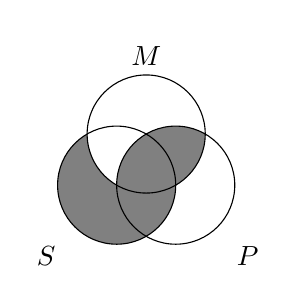
\begin{tikzpicture}
\def\firstcircle{(0,0) circle (.75cm)}
\def\secondcircle{(60:.75cm) circle (.75cm)}
\def\thirdcircle{(0:.75cm) circle (.75cm)}

\begin{scope}
\clip \thirdcircle;
\fill[gray] \secondcircle;
\end{scope}

\begin{scope}[even odd rule] % Shade P without M
\clip \secondcircle (-1,-1) rectangle (2,2);
\fill[gray] \firstcircle;
\end{scope}

\draw \firstcircle node[outer sep=.66cm, below left] {$S$};
\draw \secondcircle node [outer sep=.75cm, above] {$M$};
\draw \thirdcircle node [outer sep=.66cm, below right] {$P$};
\end{tikzpicture}
\end{center}
\end{longtabu}


\begin{exercises}
\item No $P$ are $M$, and all non-$S$ are non-$M$. Therefore some $S$ are $P$.

\answer{

Use contraposition on the minor premise to get the following

\begin{longtabu}{X[1,l,m]X[1,l,m]}

\begin{kormanize}
\premise{No $P$ are $M$
\premise{All $M$ are $S$
\vspace{-.5em}
 \item [] \rule{0.6\linewidth}{.5pt}
\item[C:] Some $S$ are $P$
 \end{kormanize}
 EAI-IV Invalid

&

\begin{venns}
\shadeintersectred{\middlecircle}{\predicatecircle}
\shadecomplementred{\middlecircle}{\middlesquare}{\subjectcircle}
\drawsubsyl
\drawmidsyl
\drawpredsyl
\end{venns}

\end{longtabu}
}


\item No $P$ are $M$, and all $S$ are $M$. Therefore all $S$ are non-$P$.
\answer{
Take the obverse of the conclusion to get:


\begin{longtabu}{X[1,l,m]X[1,l,m]}

\begin{kormanize}
\premise{No $P$ are $M$
\premise{All $S$ are $M$
\vspace{-.5em}
 \item [] \rule{0.6\linewidth}{.5pt}
\item[C:] No $S$ are $P$
 \end{kormanize}
Cesare (EAE-II) (Valid)


&
\begin{venns}
\shadeintersectred{\middlecircle}{\predicatecircle}
\shadecomplementred{\subjectcircle}{\subjectsquare}{\middlecircle}
\drawsubsyl
\drawmidsyl
\drawpredsyl
\end{venns}
\end{longtabu}

}
\item No $M$ are $P$, and some $S$ are $M$. Therefore some non-$P$ are not non-$S$.

\answer{
Take the contrapositive of the conclusion to get


\begin{longtabu}{X[1,l,m]X[1,l,m]}

\begin{kormanize}
\premise{No $M$ are $P$
\premise{Some $S$ are $M$
\vspace{-.5em}
 \item [] \rule{0.6\linewidth}{.5pt}
\item[C:] Some $S$ are not $P$
 \end{kormanize}
Ferio (EIO-I) (valid)

&
\begin{venns}
\shadeintersectred{\middlecircle}{\predicatecircle}
\someexistfive
\drawsubsyl
\drawmidsyl
\drawpredsyl
\end{venns}
\end{longtabu}
}
\item All non-$P$ are non-$M$, and some $S$ are $M$. Therefore all $S$ are $P$.

\answer{
 Perform contraposition on the major premise to get

\begin{longtabu}{X[1,l,m]X[1,l,m]}

\begin{kormanize}
\premise{All $M$ are $P$
\premise{Some $S$ are $M$
\vspace{-.5em}
 \item [] \rule{0.6\linewidth}{.5pt}
\item[C:] All $S$ are $P$
 \end{kormanize}
 AIA-I Invalid

&
\begin{venns}
\shadecomplementred{\middlecircle}{\middlesquare}{\predicatecircle}
\someexistseven
\drawsubsyl
\drawmidsyl
\drawpredsyl
\end{venns}
\end{longtabu}
}
\item All non-$M$ are non-$P$, and no $S$ are $M$. Therefore no $S$ are $P$.
\answer{
Perform contraposition on the major premise to get

\begin{longtabu}{X[1,l,m]X[1,l,m]}

\begin{kormanize}
\premise{All $P$ are $M$
\premise{No $S$ are $M$
\vspace{-.5em}
 \item [] \rule{0.6\linewidth}{.5pt}
\item[C:] No $S$ are $P$
 \end{kormanize}
Camestres (AEE-II) (valid)
%
%
&
\begin{venns}
\shadecomplementred{\predicatecircle}{\predicatesquare}{\middlecircle}
\shadeintersectred{\subjectcircle}{\middlecircle}
\drawsubsyl
\drawmidsyl
\drawpredsyl
\end{venns}
\end{longtabu}
}
\item All $P$ are $M$, and all $S$ are non-$M$. Also, some $S$ exist. Therefore, some $S$ are not $P$.
\answer{
Perform obversion on the minor premise to get

\begin{longtabu}{X[1,l,m]X[1,l,m]}

\begin{kormanize*}
\item All $P$ are $M$
\item No $S$ are $M$
\item Some $S$ exist.
\itemc Some $S$ are not $P$
\end{kormanize*}

AEO-IV (conditionally valid)

&
\begin{venns}
\shadecomplementred{\predicatecircle}{\predicatesquare}{\middlecircle}
\shadeintersectred{\subjectcircle}{\middlecircle}
\someexistone
\drawsubsyl
\drawmidsyl
\drawpredsyl
\end{venns}
\end{longtabu}
}
\item Some $P$ are not non-$M$. All non-$M$ are non-$S$. Some $S$ exist. Therefore some $S$ are $P$.
\answer{
perform obversion on the major premise and contraposition on the minor premise

\begin{longtabu}{X[1,l,m]X[1,l,m]}

\begin{kormanize}
\premise{Some $P$ are $M$
\premise{All $S$ are $M$
\item[P$_3$:] Some $S$ exist.
\vspace{-.5em}
 \item [] \rule{0.6\linewidth}{.5pt}
\item[C:] Some $S$ are $P$
 \end{kormanize}
 IAI-II Invalid

&
\begin{venns}
\SaMred
\drawsubsyl
\drawmidsyl
\drawpredsyl
\someexistsixseven
\someexistfiveseven
\end{venns}
\end{longtabu}
}

\item All non-$M$ are non-$P$, and all $S$ are non-$M$. Therefore no $S$ are $P$.
\answer{
Perform contraposition on the major premise and obversion on the minor premise to get:
\begin{longtabu}{X[1,l,m]X[1,l,m]}

\begin{kormanize}
\premise{All $P$ are $M$
\premise{No $S$ are $M$
\vspace{-.5em}
 \item [] \rule{0.6\linewidth}{.5pt}
\item[C:] No $S$ are $P$
 \end{kormanize}
Camestres (AEE-II) (valid)

%
&
\begin{venns}
\PaMred
\SeMred
\drawsubsyl
\drawmidsyl
\drawpredsyl

\end{venns}
\end{longtabu}
}
\item All $P$ are $M$, and all $M$ are non-$S$. Therefore all $P$ are non-$S$

\answer{
Take the obverse of the minor premise and the conclusion to get:

\begin{longtabu}{X[1,l,m]X[1,l,m]}
\begin{kormanize}
\premise{All $P$ are $M$
\premise{No $M$ are $S$
\vspace{-.5em}
 \item [] \rule{0.6\linewidth}{.5pt}
\item[C:] No $S$ are $P$
 \end{kormanize}
Calemes (AEE-IV) (valid)
%
&
\begin{venns}

\PaMred
\SeMred


\drawsubsyl
\drawmidsyl
\drawpredsyl

\end{venns}
\end{longtabu}
}

\item All $M$ are $P$, and some non-$M$ are not $S$. Therefore some $S$ are not non-$P$.

 \answer{Convert the minor premise to get ``Some $S$ are not non-$M$.'' Then take the obverse to get ``Some $S$ are $M$.'' Then take the obverse of the conclusion to get:

\begin{longtabu}{X[1,l,m]X[1,l,m]}

\begin{kormanize}
\premise{All $M$ are $P$
\premise{Some $S$ are $M$
\vspace{-.5em}
 \item [] \rule{0.6\linewidth}{.5pt}
\item[C:] Some $S$ are $P$
 \end{kormanize}
Darii (AII-1) (valid)


%
&
\begin{venns}
\MaPred
\someexistseven
\drawsubsyl
\drawmidsyl
\drawpredsyl

\end{venns}
\end{longtabu}
}
\end{exercises}
\noindent\problempart The following arguments are given with variables for the terms. Use obversion and contraposition to reduce the number of terms to three. State which operations you are using on which statements, and give the resulting syllogism in canonical form. Finally, use Venn diagrams to evaluate the argument.
\begin{exercises}

\item All non-$M$ are non-$P$, and no $S$ are $M$. Therefore no $S$ are $P$.

\answer{
\begin{kormanize}
\premise{All $P$ are $M$
\premise{No $S$ are $M$
\vspace{-.5em}
 \item [] \rule{0.6\linewidth}{.5pt}
\item[C:] No $S$ are $P$
 \end{kormanize}
Camestres (AEE-II) (valid)
contraposition Major premise }

\item All non-$P$ are non-$M$, and all non-$M$ are non-$S$. Therefore all $S$ are $P$.

\answer{
\begin{kormanize}
\premise{All $M$ are $P$
\premise{All $S$ are $M$
\vspace{-.5em}
 \item [] \rule{0.6\linewidth}{.5pt}
\item[C:] All $S$ are $P$
 \end{kormanize}
   }

\item All non-$M$ are non-$P$, and no $M$ are $S$. Also, some $S$ exist. Therefore some $S$ are not $P$.

\answer{
AEO-IV (conditionally valid)
contraposition Major premise
}

\item Some $M$ are $P$ and no $M$ are non-$S$. Therefore some $S$ are $P$.

\answer{
\begin{kormanize}
\premise{Some $M$ are $P$
\premise{All $M$ are $S$
\vspace{-.5em}
 \item [] \rule{0.6\linewidth}{.5pt}
\item[C:] Some $S$ are $P$
 \end{kormanize}
 IAI-III Invalid
obverse Minor premise
}

\item No $P$ are $M$, and all $M$ are non-$S$. Therefore no $S$ are $P$.

\answer{
\begin{kormanize}
\premise{No $P$ are $M$
\premise{No $M$ are $S$
\vspace{-.5em}
 \item [] \rule{0.6\linewidth}{.5pt}
\item[C:] No $S$ are $P$
 \end{kormanize}
 IAA-4
obv Minor premise
}

\item No $P$ are $M$, and all $S$ are $M$. Also some $S$ exist. Therefore some non-$P$ are not non-$S$.
\answer{EAO-1I (conditionally valid)
contraposition Conclusion }

\item All $P$ are $M$, and no $S$ are $M$. Therefore all $S$ are non-$P$.
\answer{
\begin{kormanize}
\premise{All $P$ are $M$
\premise{No $S$ are $M$
\vspace{-.5em}
 \item [] \rule{0.6\linewidth}{.5pt}
\item[C:] No $S$ are $P$
 \end{kormanize}
Camestres (AEE-II) (valid)
obverse Conclusion
 obverse Minor premise
}

\item All $M$ are $P$, and all $M$ are $S$. Also, some $M$ exist. Therefore some $S$ are not non-$P$.
\answer{
AAI-III (conditionally valid)
obverse Minor premise
 obverse Conclusion  }

\item All non-$P$ are non-$M$, and some $M$ are not $S$. Also some $M$ exist. Therefore, some non-$P$ are $S$.

\answer{
\begin{kormanize}
\premise{All $M$ are $P$
\premise{Some $M$ are not $S$
Some $M$ exist.
\vspace{-.5em}
 \item [] \rule{0.6\linewidth}{.5pt}
\item[C:] Some $S$ are not $P$
 \end{kormanize}
 AOO-III Invalid
 contraposition Conclusion  then obverse Conclusion
 contraposition major premise
}

\item All non-$M$ are non-$P$, and all $M$ are non-$S$. Therefore all $S$ are non-$M$.

\answer{
\begin{kormanize}
\premise{All $P$ are $M$
\premise{No $M$ are $S$
\vspace{-.5em}
 \item [] \rule{0.6\linewidth}{.5pt}
\item[C:] No $S$ are $P$
 \end{kormanize}
Calemes (AEE-IV) (valid)
contraposition Major premise
 obsert  minor premise
 obverse Conclusion
}


\end{exercises}



\noindent \problempart For each inference make a translation key and put the argument in standard form. If you use obversion or contraposition to reduce the number of the terms, make a note of it. Then construct a Venn diagram for it, and determine whether the inference is valid.

\begin{longtabu}{p{.1\linewidth}p{.5\linewidth}p{.4\linewidth}}
\textbf{Example}: & \multicolumn{2}{p{.9\linewidth}}{No one who studies logic is completely stupid, and some philosophers are not non-logicians. Therefore some philosophers are not completely stupid.} \\
\\
\textbf{Answer}: & $S$: Philosophers \newline
					$M$: Logicians \newline
					$P$: People who are completely stupid \newline
					Obversion on the minor premise

&
\vspace{-16pt}
\begin{kormanize}
\premise{No $M$ are $P$.
\premise{Some $S$ are $M$.
\conclusion{Some $S$ are not $P$.
\end{kormanize} \\

&
\vspace{-28pt}
\begin{center}
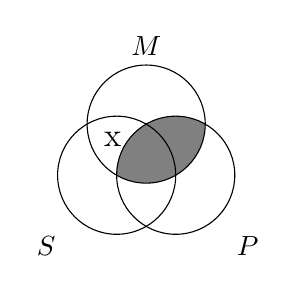
\begin{tikzpicture}
\def\firstcircle{(0,0) circle (.75cm)}
\def\secondcircle{(60:.75cm) circle (.75cm)}
\def\thirdcircle{(0:.75cm) circle (.75cm)}

\begin{scope} %shade overlap between S and M
\clip \thirdcircle;
\fill[gray] \secondcircle;
\end{scope}

\draw \secondcircle node [outer sep=.75cm, above] {$M$};
\draw \thirdcircle node [outer sep=.66cm, below right] {$P$};
\draw \firstcircle node[outer sep=.66cm, below left] {$S$}
	node [xshift=-.05cm, yshift=.45cm](5){\large{x}};
\end{tikzpicture}
\end{center}

& Ferio (EIO-1) \newline Unconditionally valid

\end{longtabu}

%No food is inedible. In fact, all food is edible. Therefore nothing this is inedible is edible.

\begin{exercises}

\item All of Lorain County is outside of Cuyahoga County, but at least some of Cleveland is in Cuyahoga County. Therefore some of Lorain County is not in Cleveland.

\answer{

\begin{longtabu}{X[1,l,p]X[1,l,p]}

\begin{description}
\item[$S$:] Places in Lorain County
\item[$M$:] Places in Cuyahoga County
\item[$P$:] Places in Cleveland
\end{description}

&

\begin{kormanize}
\premise{Some $P$ are $M$
\premise{No $S$ are $M$  %All $S$ are non-$M$
\vspace{-.5em}
 \item [] \rule{0.6\linewidth}{.5pt}
\item[C:] Some $S$ are not $P$
 \end{kormanize}
IEO-II (Invalid)

\end{longtabu}
}

\item All Civics are vehicles. After all, any automobile is a vehicle, and a Civic is a kind of car.

\answer{
\begin{longtabu}{X[1,l,p]X[1,l,p]}

\begin{description}
\item[$S$:] Civics
\item[$M$:] Car (or automobile)
\item[$P$:] Vehicle.
\end{description}

&

\begin{kormanize}
\premise{All $M$ are $P$
\premise{All $S$ are $M$
\vspace{-.5em}
 \item [] \rule{0.6\linewidth}{.5pt}
\item[C:] All $S$ are $P$
 \end{kormanize}
Barbara (AAA-I) (valid)

\end{longtabu}
}

\item Cows are animals. After all, anything that is not an animal is also not a farm animal, and cows are farm animals.

\answer{
\begin{longtabu}{X[1,l,p]X[1,l,p]}

\begin{description}
\item[$S$:] Cows
\item[$M$:] Farm animals
\item[$P$:] Animals
\end{description}
 Contrapose major premise.
&

\begin{kormanize*}
\item All $M$ are $P$
\item All $S$ are $M$
\itemc All $S$ are $P$
\end{kormanize*}


Barbara (AAA-1) (Valid.)

  \end{longtabu}
}

\item Some digits are fingers, and if something is a digit, then it is a body part. Therefore some body parts are non-fingers.

\answer{
\begin{longtabu}{X[1,l,p]X[1,l,p]}

\begin{description}
\item[$S$:] Body Parts
\item[$M$:] Digits
\item[$P$:] Fingers
\end{description}

Contrapose minor premise, obvert conclusion.

&


\begin{kormanize}
\premise{Some $M$ are $P$
\premise{All $M$ are $S$
\vspace{-.5em}
 \item [] \rule{0.6\linewidth}{.5pt}
\item[C:] Some $S$ are not $P$
 \end{kormanize}
 IAO-III Invalid

\end{longtabu}
}

\item Earth is a planet. Therefore Earth is not a moon, because no planets are moons.

\answer{
\begin{longtabu}{X[1,l,p]X[1,l,p]}

\begin{description}
\item[$S$:] Things identical to the Earth
\item[$M$:] Planet
\item[$P$:] Moon
\end{description}

&

\begin{kormanize}
\premise{No $M$ are $P$
\premise{All $S$ are $M$
\vspace{-.5em}
 \item [] \rule{0.6\linewidth}{.5pt}
\item[C:] No $S$ are $P$
 \end{kormanize}
Celarent (EAE-I) (valid)

\end{longtabu}
}

\item All trees are non-animals. Some trees are deciduous. Therefore some non-animals are not evergreen.

\answer{
\begin{longtabu}{X[1,l,p]X[1,l,p]}

\begin{description}
\item[$S$:] Deciduous trees.
\item[$M$:] Trees.
\item[$P$:] Animals.
\end{description}

Obvert major premise, convert evergreen to non-deciduous, contrapose conclusion

&

\begin{kormanize}
\premise{No $P$ are $M$
\premise{Some $M$ are $S$
\vspace{-.5em}
 \item [] \rule{0.6\linewidth}{.5pt}
\item[C:] Some $S$ are not $P$
 \end{kormanize}
Fresison (EIO-IV) (valid)

\end{longtabu}
}

\item Some relatives are not blood relatives, and some in-laws are mothers-in-law. Therefore, some non-relatives are not non-mothers-in-law.

\answer{

\begin{longtabu}{X[1,l,p]X[1,l,p]}

\begin{description}
\item[$S$:] Mothers-in-law
\item[$M$:] In-laws
\item[$P$:] Relatives
\end{description}

In the major premise, change ``not blood relatives'' to ``in laws'' and then contrapose the conclusion.

&

\begin{kormanize}
\premise{Some $P$ are $M$
\premise{Some $M$ are $S$
\vspace{-.5em}
 \item [] \rule{0.6\linewidth}{.5pt}
\item[C:] Some $S$ are not $P$
 \end{kormanize}
 IIO-IV Invalid

\end{longtabu}
}

\item Ludwig Wittgenstein was not English. Therefore Ludwig Wittgenstein was a philosopher, because some English people are philosophers.

\answer{
\begin{longtabu}{X[2,l,p]X[1,l,p]}

\begin{description}
\item[$S$:] People identical to Ludwig Wittgenstein
\item[$M$:] Philosophers
\item[$P$:] People who are English
\end{description}

&

\begin{kormanize}
\premise{Some $M$ are $P$
\premise{No $S$ are $M$
\vspace{-.5em}
 \item [] \rule{0.6\linewidth}{.5pt}
\item[C:] All $S$ are $P$
 \end{kormanize}
 IEA-I Invalid
\end{longtabu}
}

\item Some liquids are non-alcoholic. This is because only liquids are drinks, and some non-alcoholic things are not non-drinks.

\answer{
\begin{longtabu}{X[1,l,p]X[1,l,p]}

\begin{description}
\item[$S$:] Liquids
\item[$M$:] Drinks
\item[$P$:] Alcoholic liquids
\end{description}

Obvert the conclusion and take the contraposition of the minor premise

&



\begin{kormanize}
\premise{Some $M$ are not $P$
\premise{All $M$ are $S$
\vspace{-.5em}
 \item [] \rule{0.6\linewidth}{.5pt}
\item[C:] Some $S$ are not $P$
 \end{kormanize}
 OAO-III Bocardo, Valid.
\end{longtabu}
}

\item No advertisements are misleading. Therefore all pandering things are non-misleading, because no advertisements are pandering.

\answer{
\begin{longtabu}{X[1,l,p]X[1,l,p]}

\begin{description}
\item[$S$:] Things that pander.
\item[$M$:] Advertisements
\item[$P$:] Misleading things
\end{description}

Obvert the conclusion.

&



\begin{kormanize}
\premise{No $M$ are $P$
\premise{No $M$ are $P$
\vspace{-.5em}
 \item [] \rule{0.6\linewidth}{.5pt}
\item[C:] No $S$ are $P$
 \end{kormanize}
 EEE-I Invalid
\end{longtabu}
}


\end{exercises}
\noindent \problempart For each inference make a translation key and put the argument in standard form. Then construct a Venn diagram for it and determine whether the inference is valid.


\begin{exercises}

\item Some machines are likely to break, because some machines are elaborate, and nothing that is elaborate is unlikely to break.

\answer{
\begin{kormanize}
\premise{All $M$ are $P$
\premise{Some $S$ are $M$
\vspace{-.5em}
 \item [] \rule{0.6\linewidth}{.5pt}
\item[C:] Some $S$ are $P$
 \end{kormanize}
Darii (AII-1) (valid)
 obvert major premise
}

\item Only mammals are dogs, and no mammals are reptiles. Also, \emph{Canis familiaris} really do exist. Therefore some dogs are not reptiles.


\answer{
\begin{kormanize}
\premise{All $P$ are $M$
\premise{No $M$ are $S$
\item[{\color{red}P$_3$:}] {\color{red}Some $S$ exist.}
\conclusion{Some $S$ are not $P$
\end{kormanize}

AEO-IV (conditionally valid)
 exclusive propositions
 }


\item All of Ohio is in the United States. Therefore none of Ohio is in Canada, because no part of Canada is in the United States.
\answer{Camestres (AEE-II) (unconditionally valid) }



\item All sneeps are snine. This is because all non-snine things are also non-sneeps, and all sneeps are snine.

\answer{
\begin{description}
\item[$S$:] Snerps
\item[$M$:] Sneeps
\item[$P$:] Snine things
\end{description}

\begin{kormanize}
\premise{All $M$ are $P$
\premise{All $S$ are $M$
\vspace{-.5em}
 \item [] \rule{0.6\linewidth}{.5pt}
\item[C:] All $S$ are $P$
 \end{kormanize}
Barbara (AAA-I) (valid)
 implicit noun phrases
}

\item No non-forks are pointy. Therefore, all pointy things are forks, because no pointy things are non-forks.

\answer{
\begin{description}
\item[$S$:] Utensils.
\item[$M$:] Pointy things
\item[$P$:] Forks
\end{description}


\begin{kormanize}
\premise{All $M$ are $P$
\premise{Some $S$ are $M$
\vspace{-.5em}
 \item [] \rule{0.6\linewidth}{.5pt}
\item[C:] Some $S$ are $P$
 \end{kormanize}
Darii (AII-1) (valid)
 nonstandard verbs
obverse Conclusion
 obverse Minor premise
}

\item Some arguments are not invalid. After all, anything that is persuasive is valid, and anything that is persuasive is also an argument. Furthermore, we know that some arguments exist.

\answer{
\begin{kormanize*}
\item All $M$ are $P$
\item All $M$ are $S$
\item Some $S$ exist.
\itemc Some $S$ are $P$
\end{kormanize*}
AAI-III (conditionally valid)
}


\item Some things that sing don't sink in water. You can tell because some bricks do not sing, and all bricks float.

\answer{
\begin{kormanize}
\premise{Some $M$ are not $P$
\premise{All $M$ are $S$
\vspace{-.5em}
 \item [] \rule{0.6\linewidth}{.5pt}
\item[C:] All $S$ are $P$
 \end{kormanize}
 OAA-III Invalid

}


\item Crayons are not precision tools. Therefore all toys are non-precision tools, because some toys are crayons.

\answer{
\begin{kormanize}
\premise{No $M$ are $P$
\premise{Some $S$ are $M$
\vspace{-.5em}
 \item [] \rule{0.6\linewidth}{.5pt}
\item[C:] No $S$ are $P$
 \end{kormanize}
 EIE-1 Invalid
 obverse Conclusion
 contraposition Major premise
}



\item  Some things that aren't beliefs are not objectionable. This is because all things that are not well founded are non-beliefs, and all things that are well founded are unobjectionable.

\answer{
\begin{description}
\item[$S$:] objectionable.
\item[$M$:]  Well-founded
\item[$P$:] Beliefs
\end{description}

AEO-IV (conditionally valid)

\begin{kormanize*}
\item All $P$ are $M$
\item  No $M$ are $S$
\itemc  Some $S$ are not $P$
\end{kormanize*}
}

\item Some Kaiju are not characters from Toho studios. Therefore Godzilla is not a Kaiju, because Godzilla is a character from Toho studios.

\answer{
\begin{kormanize}
\premise{Some $P$ are not $M$
\premise{All $S$ are $M$
\vspace{-.5em}
 \item [] \rule{0.6\linewidth}{.5pt}
\item[C:] No $S$ are $P$
 \end{kormanize}
 OAE-II Invalid
}


\end{exercises}


\practiceproblems
\noindent \problempart Write each enthymeme below in standard form and supply the premise or conclusion that makes the argument valid, marking it with an asterisk. If no statement can make the argument valid, write ``invalid.''

\begin{longtabu}{p{.1\linewidth}p{.9\linewidth}}
\textbf{Example}: & Edinburgh is in Scotland, and no part of Scotland is sunny. \\
\textbf{Answer}: &
\vspace{-16pt}
\begin{kormanize}
\premise{All places in Edinburgh are places in Scotland.
\premise{No places in Scotland are places that are sunny.
\conclusion{No places in Edinburgh are sunny.*
\end{kormanize}
\end{longtabu}


%Version of the example with context.

%\begin{longtabu}{p{.1\linewidth}p{.1\linewidth}p{.8\linewidth}}
%\textbf{Example}: & \multicolumn{2}{p{.9\linewidth}}{\textit{Steve and Monica are considering where to go on their vacation.}} \\
%&\textbf{Steve}: &Is Edinburgh sunny? \\
%&\textbf{Monica}: &Well, Edinburgh is in Scotland, and no part of Scotland is sunny. Do you think it is sunny?\\
%\textbf{Answer}: &
%\multicolumn{2}{p{.9\linewidth}}{
%\vspace{-16pt}
%\begin{kormanize}
%\premise{All places in Edinburgh are places in Scotland.
%\premise{No places in Scotland are places that are sunny.
%\vspace{-.5em}
%\item [] \rule{0.6\linewidth}{.5pt}
%\item[C:] No places in Edinburgh are sunny.*
%\end{kormanize}
%}
%\end{longtabu}

\begin{exercises}
\item Dogs are mammals, which means that they aren't reptiles.

\answer{
\begin{kormanize*}
\item No reptiles are mammals*
\item All dogs are mammals
\itemc[.3] No dogs are reptiles
 \end{kormanize*}
Cesare (EAE-2)
}

\item Some pastas must be whole wheat, because some linguine is whole wheat.
\answer{
\begin{kormanize*}
\item All linguine is pasta*
\item Some linguine is whole wheat
\itemc[.3] Some pastas are whole wheat
\end{kormanize*}
Datisi (AII-3)
}


\item If you have ten dollars, you can see the movie. So therefore none of the kids will see the movie.

\answer{
Not valid. \vspace{6pt}\\
If you change the if-then statement into the appropriate mood A statement, you get ``All people who have ten dollars can see the movie,'' but there is no way to get from there to the conclusion ``No kids will see the movie.''

\begin{kormanize*}
\item All people who have ten dollars are people who can see the movie
\item ?
\itemc No kids are people who can see the movie
\end{kormanize*}
A?E-1 or -3 \vspace{6pt}\\
To make the argument work, you would need to have ``All people who can see the movie are people who have ten dollars'' as the major premise.
}


\item Nothing divine is evil, so no gods are evil.

\answer{
\begin{kormanize*}
\item All Gods are divine things*
\item No divine things are evil
 \itemc[.2] No Gods are evil
 \end{kormanize*}
Calemes (AEE-IV) (valid)
}

\item No logicians are ignorant of Aristotle, and some people who are ignorant of Aristotle are foolish.
\answer{
\begin{kormanize*}
\item No logicians are people who are ignorant of Aristotle.
\item Some people who are ignorant of Aristotle are foolish people
\itemc[.3] Some foolish people are not logicians*'
 \end{kormanize*}
Fresison (EIO-IV)
}


\item No holidays are work days, and some work days are not Mondays.

\answer{
Not valid \vspace{6pt}
\begin{kormanize*}
\item No holidays are work days.
\item Some work days are not Mondays.
\itemc ?
\end{kormanize*}
EO?-?
}

\item Some trees are not evergreens. Therefore some evergreens are not spruces.

\answer{
Not valid \vspace{6pt}
\begin{kormanize*}
\item ?
\item Some trees are not evergreens
\itemc[.2] Some evergreens are not spruces
 \end{kormanize*}
?OO-3 or -4
}

\item No jellyfish are vertebrates, but some animals that make good pets are vertebrates.
\answer{
\begin{kormanize*}
\item No jellyfish are vertebrates
\item Some animals that make good pets are vertebrates
\itemc[.2] Some animals that make good pets are not jellyfish*
 \end{kormanize*}
Festino (EIO-II)}

\item Some chairs are not houses, and all tables are houses.
\answer{
\begin{kormanize*}
\item All tables are houses
\item Some chairs are not houses
\itemc[.4] Some chairs are not tables*
 \end{kormanize*}
Baroco (AOO-2) \vspace{6pt} \\
This is a little tricky, because you have to switch the order of the two premises from the way they are given in the problem. If you don't, ``tables'' has to be the subject of the conclusion and ``chairs'' has to be the predicate, and there is nothing you can with the terms in that order.
}


\item No doodlebugs are octofish. Therefore no thing-havers are octofish.

\answer{
\begin{kormanize*}
\item No doodlebugs are octofish
\item All thing-havers are doodlebugs
\itemc[.4] No thing-havers are octofish
 \end{kormanize*}
Celarent (EAE-I)
}




\end{exercises}

\noindent \problempart Write each enthymeme below in standard form and supply the premise or conclusion that makes the argument valid, marking it with an asterisk. If no statement can make the argument valid, write ``invalid.''

\begin{exercises}
\item No board games are online games, because all online games are video games.

%\begin{kormanize}
%\premise{No $M$ are $P$
%\premise{All $S$ are $M$
%\vspace{-.5em}
% \item [] \rule{0.6\linewidth}{.5pt}
%\item[C:] No $S$ are $P$
% \end{kormanize}
%Celarent (EAE-I) (valid)
%nonstandard quantifiers
%Delete Major premise

\item No coins are paper money. Therefore no coins are two dollar bills.
%\begin{kormanize}
%\premise{All $P$ are $M$
%\premise{No $S$ are $M$
%\vspace{-.5em}
% \item [] \rule{0.6\linewidth}{.5pt}
%\item[C:] No $S$ are $P$
% \end{kormanize}
%Camestres (AEE-II) (valid)
%exclusive propositions
%Delete Major premise


\item Some vegetables are peppers. Therefore some foods are peppers.

%\begin{kormanize}
%\premise{Some $M$ are $P$
%\premise{All $M$ are $S$
%\vspace{-.5em}
% \item [] \rule{0.6\linewidth}{.5pt}
%\item[C:] Some $S$ are $P$
% \end{kormanize}
%Disamis (IAI-III) (valid)
%adverbs and pronouns
%Delete Minor premise


\item Everyone who fights for justice is a saint. Therefore no politicians are saints.
%
%\begin{kormanize}
%\premise{All justice fighters are saints
%\premise{No politicians are justice fighters*
%\vspace{-.5em}
% \item [] \rule{0.6\linewidth}{.5pt}
%\item[C:] No politicians are saints
% \end{kormanize}
% AEE-I----looks like celarent, but

%invalid

\item Some children are not getting treats because no one who was naughty gets treats.

%\begin{kormanize}
%\premise{No $M$ are $P$
%\premise{Some $S$ are $M$
%\vspace{-.5em}
% \item [] \rule{0.6\linewidth}{.5pt}
%\item[C:] Some $S$ are not $P$
% \end{kormanize}
%Ferio (EIO-I) (valid)nonstandard quantifiers
%Delete Minor premise


\item On days when there is more than a foot of snow, school is canceled. Therefore some Mondays this winter school will be canceled.

%\begin{kormanize}
%\premise{All $M$ are $P$
%\premise{Some $S$ are $M$
%\vspace{-.5em}
% \item [] \rule{0.6\linewidth}{.5pt}
%\item[C:] Some $S$ are $P$
% \end{kormanize}
%Darii (AII-1) (valid) conditional statements
%Delete Minor premise



\item All churches are religious institutions. Therefore, some churches are not Christian.
%\begin{kormanize}
%\premise{Some $M$ are not $P$
%\premise{All $S$ are $M$
%\vspace{-.5em}
% \item [] \rule{0.6\linewidth}{.5pt}
%\item[C:] Some $S$ are not $P$
% \end{kormanize}
%invalid

\item All rocks are food, and some vegetables are rocks.
%\begin{kormanize}
%\premise{All $M$ are $P$
%\premise{Some $S$ are $M$
%\vspace{-.5em}
% \item [] \rule{0.6\linewidth}{.5pt}
%\item[C:] Some $S$ are $P$
% \end{kormanize}
%Darii (AII-1) (valid)
%the only
%Delete Conclusion



\item Some houses are not offices, and some residences are not offices.
%
%\begin{kormanize}
%\premise{Some $P$ are not $M$
%\premise{All $M$ are $S$
%\vspace{-.5em}
% \item [] \rule{0.6\linewidth}{.5pt}
%\item[C:] Some $S$ are not $P$
% \end{kormanize}

%invalid.


\item No snirt are hirt. Therefore some blorp are not snirt.
%\begin{kormanize}
%\premise{No $P$ are $M$
%\premise{Some $S$ are $M$
%\vspace{-.5em}
% \item [] \rule{0.6\linewidth}{.5pt}
%\item[C:] Some $S$ are not $P$
% \end{kormanize}
%Festino (EIO-II) (valid)
%nonstandard verbs
%Delete Minor premise

\end{exercises}

\practiceproblems

\noindent\problempart \label{venn_set1} Rewrite the following arguments in standard form, reducing the number of terms if necessary. Then supply the missing intermediate conclusions and evaluate the arguments with Venn diagrams.

\begin{longtabu}{{X[1,l,p]X[9,l,p]}}
\textbf{Example}: &
\vspace{-16pt}
\begin{kormanize}
\premise{No $D$ are non-$B$.
\premise{All $B$ are $A$.
\premise{No $A$ are $C$.
\conclusion{Some $D$ are not $C$.
\end{kormanize}
\\
\textbf{Answer}: & Standard form:  \begin{kormanize}
\premise{No $A$ are $C$.
\premise{All $B$ are $A$. % No $C$ are $A$
\premise{All $D$ are $B$.
\conclusion{Some $D$ are not $C$.
\end{kormanize}\\

&

\begin{tikzpicture}%
%%%% Venn 1
\begin{scope}
\def\firstcircle{(0,0) circle (.75cm)}
\def\secondcircle{(60:.75cm) circle (.75cm)}
\def\thirdcircle{(0:.75cm) circle (.75cm)}

\begin{scope} %shade overlap between S and M
\clip \thirdcircle;
\fill[gray] \secondcircle;
\end{scope}

\begin{scope}[even odd rule] % Shade P without M
\clip \secondcircle (-1,-1) rectangle (2,2);
\fill[gray] \firstcircle;
\end{scope}

\draw \firstcircle node[outer sep=.66cm, below left] {$B$};
\draw \secondcircle node [outer sep=.75cm, above] {$A$};
\draw \thirdcircle node [outer sep=.66cm, below right] {$C$};
\end{scope}


%%%% Venn 2
\begin{scope}[shift={(4.25cm,0cm)}]
\def\firstcircle{(0,0) circle (.75cm)}
\def\secondcircle{(60:.75cm) circle (.75cm)}
\def\thirdcircle{(0:.75cm) circle (.75cm)}

\begin{scope} %shade overlap between S and M
\clip \thirdcircle;
\fill[gray] \secondcircle;
\end{scope}

\begin{scope}[even odd rule] % Shade P without M
\clip \secondcircle (-1,-1) rectangle (2,2);
\fill[gray] \firstcircle;
\end{scope}

\draw \firstcircle node[outer sep=.66cm, below left] {$D$};
\draw \secondcircle node [outer sep=.75cm, above] {$B$};
\draw \thirdcircle node [outer sep=.66cm, below right] {$C$};
\end{scope}

%%%%%%%%%%%% Arg 1
 \node at (0,-2.65) [text width=4.5cm, outer sep=1mm] (Cesare){
\begin{kormanize}
\premise{No $A$ are $C$.
\premise{All $B$ are $A$.
\conclusion{No $B$ are $C$.
\end{kormanize}
};

%%%%%%%%%%%% Arg 2
\node at (5.25,-2.5)[text width=4.5cm, outer sep=1mm] (Ferison){
\begin{kormanize}
\premise{No $B$ are $C$.
\premise{All $D$ are $B$.
\vspace{-.5em}
\item [] \rule{0.9\linewidth}{.5pt}
\item[C:] Some $D$ are not $C$.
\end{kormanize}
};

\draw [myarrow1, ->] (1, -3.3) .. controls (2.125, -3.3) and (2.125, -2.15) .. (3.15, -2.15);

\node at (0,-4){\textbf{Celarent (EAE-I)}};
\node at (5,-4) {\textbf{Celaront (EAO-1)}};

\end{tikzpicture}

\\
& Conditionally valid. It also needs the premise ``Some $D$ exist.''

\end{longtabu}

\begin{exercises}

\begin{longtabu}{X[1,p,m]X[1,p,m]}

\item \begin{kormanize}
\premise{All $B$ are $A$.
\premise{Some $C$ are $D$.
\premise{No $D$ are $A$.
\conclusion{Some $C$ are not $B$.
 \end{kormanize}

%\begin{kormanize}
%\premise{All $B$ are $A$
%\premise{No $D$ are $A$ %No $D$ are $B$
%\premise{Some $C$ are $D$
%\vspace{-.5em}
% \item [] \rule{0.2\linewidth}{.5pt}
%\item[C:] Some $C$ are not $B$
% \end{kormanize}

% A --> B
% B --> A
% C --> D
% D --> C

&

\item \begin{kormanize}
\premise{Some $B$ are $C$.
\premise{All $D$ are $A$.
\premise{Some $C$ are $D$.
\conclusion{All $A$ are $B$.
 \end{kormanize}

%\begin{kormanize}
%\premise{Some $B$ are $C$
%\premise{Some $C$ are $D$
%\premise{All $D$ are $A$
%\vspace{-.5em}
% \item [] \rule{0.2\linewidth}{.5pt}
%\item[C:] All $A$ are $B$
% \end{kormanize}

% A --> B
% B --> C
% C --> D
% D --> A

\\

\item \begin{kormanize}
\premise{All $B$ are $C$.
\premise{Some $B$ are $A$. %Some $B$ are not $D$
\premise{All $D$ are non-$A$. %becomes No $D$ are $A$
\conclusion{Some $C$ are not $D$.
 \end{kormanize}

% \begin{kormanize}
%\premise{All $A$ are non-$B$ %becomes No $A$ are $B$
%\premise{Some $C$ are $B$ %Some $C$ are not $A$
%\premise{All $C$ are $D$
%\vspace{-.5em}
% \item [] \rule{0.2\linewidth}{.5pt}
%\item[C:] Some $D$ are not $A$.
% \end{kormanize}

% A --> D
% B --> A
% C --> B
% D --> C

%Festino (EIO-II), Bocardo (OAO-3)

&

\item \begin{kormanize}
\premise{No $A$ are $B$.
\premise{No $C$ are $B$. % No $B$ are $E$
\premise{All $D$ are $A$.
\premise{All $E$ are $C$.
\conclusion{No $D$ are $E$.
 \end{kormanize}

%\begin{kormanize}
%\premise{All $E$ are $C$
%\premise{No $C$ are $B$ % No $B$ are $E$
%\premise{No $A$ are $B$
%\premise{All $D$ are $A$
%\vspace{-.5em}
% \item [] \rule{0.2\linewidth}{.5pt}
%\item[C:] No $D$ are $E$.
% \end{kormanize}

% A --> E
% B --> C
% C --> B
% D --> A
% E --> D

\\

\item \begin{kormanize}
\premise{All $A$ are $E$.
\premise{All $E$ are $D$. % All $E$ are $C$
\premise{All $A$ are $B$.
\premise{All $D$ are $C$.
\conclusion{All $B$ are $C$.
 \end{kormanize}

% A --> C
% B --> D
% C --> E
% D --> A
% E --> B

%\item \begin{kormanize}
%\premise{All $D$ are $C$
%\premise{All $E$ are $D$ % All $E$ are $C$
%\premise{All $A$ are $E$
%\premise{All $A$ are $B$
%\vspace{-.5em}
% \item [] \rule{0.2\linewidth}{.5pt}
%\item[C:] All $B$ are $C$.
% \end{kormanize}

&

\item \begin{kormanize}
\premise{All $A$ are $E$. % All $A$ are $D$
\premise{All $E$ are $D$.
\premise{Some $B$ are $C$.
\premise{All $B$ are $A$.
\conclusion{Some $C$ are $D$.
 \end{kormanize}

%\item \begin{kormanize}
%\premise{All $E$ are $D$
%\premise{All $A$ are $E$ % All $A$ are $D$
%\premise{All $B$ are $A$
%\premise{Some $B$ are $C$
%\vspace{-.5em}
% \item [] \rule{0.2\linewidth}{.5pt}
%\item[C:] Some $C$ are $D$.
% \end{kormanize}

% A --> D
% B --> E
% C --> A
% D --> B
% E --> C

\\

\item \begin{kormanize}
\premise{All $A$ are $B$.
\premise{No $C$ are $E$.
\premise{No $D$ are non-$A$.	%Some $A$ are not $C$
\premise{Some $E$ are $D$. %Some $D$ are not $C$
\conclusion{Some $B$ are not $C$.
 \end{kormanize}

%\begin{kormanize}
%\premise{No $C$ are $E$
%\premise{Some $E$ are $D$ %Some $D$ are not $C$
%\premise{No $D$ are non-$A$	%Some $A$ are not $C$
%\premise{All $A$ are $B$
%\vspace{-.5em}
% \item [] \rule{0.6\linewidth}{.5pt}
%\item[C:] Some $B$ are not $C$
% \end{kormanize}

% A --> C
% B --> E
% C --> D
% D --> A
% E --> B

&

\item \begin{kormanize}
\premise{All $D$ are $A$. % Some $A$ are not $E$
\premise{All $A$ are $C$.
\premise{All $E$ are $B$.
\premise{Some $D$ are not $B$. %  Some $D$ are not $E$
\conclusion{Some $C$ are not $E$.
 \end{kormanize}

%\begin{kormanize}
%\premise{All $E$ are $B$
%\premise{Some $D$ are not $B$ %  Some $D$ are not $E$
%\premise{All $D$ are $A$ % Some $A$ are not $E$
%\premise{All $A$ are $C$
%\vspace{-.5em}
% \item [] \rule{0.2\linewidth}{.5pt}
%\item[C:] Some $C$ are not $E$
% \end{kormanize}

% A --> E
% B --> B
% C --> D
% D --> A
% E --> C

\\

\item \begin{kormanize}
\premise{All $E$ are $D$. %  Some $D$ are not $F$
\premise{No $E$ are $F$.
\premise{All $B$ are $A$.
\premise{All $C$ are $B$.
\item[P$_5$:] All $D$ are $C$.
\conclusion{Some $A$ are not $F$.
 \end{kormanize}

 % A --> F
% B --> E
% C --> D
% D --> C
% E --> B
% F --> A
% 5 term conditionally valid.
&

\item \begin{kormanize}
\premise{All $B$ are $A$.
\premise{Some $C$ are $E$. %  Some $C$ are $F$
\premise{No $A$ are $D$.
\premise{All $C$ are $B$.%   %
\item[P$_5$:] All $E$ are $F$.
\conclusion{Some $D$ are $F$.
 \end{kormanize}
%5 premises term reduction invalid 2
% A --> F
% B --> E
% C --> C
% D -->B
% E --> A
% F --> D

\end{longtabu}

\end{exercises}

\noindent\problempart \label{venn_set2} Rewrite the following arguments in standard form, reducing the number of terms if necessary. Then supply the missing intermediate conclusions and evaluate the arguments with Venn diagrams.

\begin{exercises}
\begin{longtabu}{X[1,p,m]X[1,p,m]}
\item \begin{kormanize}
\premise{No $D$ are $C$.
\premise{No $A$ are $B$.
\premise{Some $D$ are $A$ %Some $D$ are not $B$
\conclusion{Some $C$ are not $B$.
\end{kormanize}
%3 premise, invalid

% * P --> B
% * M --> A
% * M2 --> D
% * S --> C

&
\item \begin{kormanize}
\premise{All $C$ are $B$.
\premise{No $B$ are $D$. %  No $D$ are $C$
\premise{All $A$ are $D$.
\conclusion{Some $A$ are not $C$.
\end{kormanize}
%3 premise, conditionally valid--EA family

% * P -->  C
% * M --> B
% * M2 --> D
% * S --> A

\\
\item \begin{kormanize}
\premise{Some $M$ are not $P$.
\premise{No $M$ are non-$M2$. % Some M2 are not $P$
\premise{No $M2$ are non-$S$.
\conclusion{Some $S$ are not $P$.
\end{kormanize}
%3 premise, reduce terms

% * P --> D
% * M --> C
% * M2 --> B
% * S --> A

&
\item \begin{kormanize}
\premise{All $A$ are $B$. %some $A$ are $C$
\premise{All $E$ are $A$.
\premise{All $D$ are $C$.
\premise{All $D$ are $B$. % Some $B$ are $C$
\conclusion{Some $E$ are $C$.
\end{kormanize}
%4 premise, conditionally valid--AI family

% * P --> C
% * M --> D
% * M2 --> B
% * M3 --> A
% * S --> E
\\
\item \begin{kormanize}
\premise{Some $E$ are $C$. % Some $C$ are $D$
\premise{Some $A$ are $C$.
\premise{All $B$ are $D$.
\premise{All $E$ are $B$.	%All $E$ are $D$
\conclusion{Some $A$ are $D$.
\end{kormanize}
%4 premise

% * P --> D
% * M --> B
% * M2 --> E
% * M3 --> C
% * S --> A

&
\item \begin{kormanize}
\premise{No $B$ are $C$.
\premise{Some $B$ are not $A$. % Some $B$ are not $E$
\premise{All $C$ are $D$.
\premise{All $E$ are $A$.
\conclusion{Some $D$ are not $E$.
\end{kormanize}
%4 premise, invalid

% * P --> E
% * M --> A
% * M2 --> B
% * M3 --> C
% * S --> D

\\
\item \begin{kormanize}
\premise{All $D$ are $A$.
\premise{All $C$ are $D$.
\premise{No $E$ are $B$.
\premise{No $B$ are $A$.
\conclusion{No $C$ are $E$.
\end{kormanize}
%4 premise, invalid

% * P --> E
% * M --> B
% * M2 --> A
% * M3 --> D
% * S --> C

&
\item \begin{kormanize}
\premise{No $A$ are non-$D$.
\premise{No $D$ are $C$. %No $C$ are $A$
\premise{All $B$ are $C$. %No $B$ are $A$
\premise{All non-$B$ are non-$E$
\conclusion{No $E$ are $A$.
\end{kormanize}
%4 premise, reduce terms

% * P --> A
% * M --> D
% * M2 --> C
% * M3 --> B
% * S --> E

\\
\item \begin{kormanize}
\premise{No $E$ are $F$.
\premise{All $D$ are $B$. % All $D$ are $A$
\premise{All $C$ are $E$.
\premise{Some $D$ are not $F$.
\item[P$_5$:] All $B$ are $A$.
\conclusion{Some $C$ are not $A$.
\end{kormanize}
%5 premise, invalid

% * P --> A
% * M --> B
% * M2 --> D
% * M3 --> F
% * M4 --> E
% * S --> C

&
\item \begin{kormanize}
\premise{No $B$ are $D$.
\premise{All $E$ are $A$.
\premise{All $F$ are $C$. %All $F$ are $A$
\premise{All $C$ are $E$. % All $C$ are $A$
\item[P$_5$:] All $D$ are $F$. % All $D$ are $A$
\conclusion{No $B$ are $A$.
\end{kormanize}
%5 premise, reduce terms

% * P --> A
% * M --> E
% * M2 --> C
% * M3 --> F
% * M4 --> D
% * S --> B

\end{longtabu}
\end{exercises}

\noindent\problempart Do the exercises in Part \ref{venn_set1}, but skip writing out the missing intermediate conclusions, and evaluate them using the rules method instead of the Venn diagram method.

\begin{longtabu}{p{.1\linewidth}p{.9\linewidth}}

\textbf{Example}: & \vspace{-16pt} \begin{kormanize}
\premise{No $D$ are non-$B$.
\premise{All $B$ are $A$.
\premise{No $A$ are $C$.
\conclusion{Some $D$ are not $C$.
\end{kormanize} \\
\textbf{Answer}: & \vspace{-16pt} \begin{kormanize}
\premise{No $A$\textsuperscript{D} are $C$\textsuperscript{D}.
\premise{All $B$\textsuperscript{D} are $A$. % No $C$ are $A$
\premise{All $D$\textsuperscript{D} are $B$.
\conclusion{Some $D$ are not $C$\textsuperscript{D}.
\end{kormanize}
\\ &
\textbf{Rule 1:} Pass. Middle terms $A$ and $B$ are distributed in P$_1$ and P$_2$. \newline
\textbf{Rule 2:} Pass. The conclusion distributes $C$, which is also distributed in  P$_1$.\newline
\textbf{Rule 3:} Pass. There is one negative premise, P$_1$. \newline
\textbf{Rule 4:} Pass. The conclusion is negative, and there is exactly one negative premise.\newline
\textbf{Rule 5:} Fail. The premises are all universal and the conclusion is particular. \\
& Conditionally valid. It needs the premise ``Some $D$ exist.''
\end{longtabu}


\noindent\problempart Do the exercises in Part \ref{venn_set2}, but skip writing out the missing intermediate conclusions, and evaluate them using the rules method instead of the Venn diagram method.


\noindent\problempart  Rewrite the following arguments in standard form, reducing terms if necessary, and then prove that they are valid using a single, four-term Venn diagram.

\begin{longtabu}{p{.1\linewidth}p{.8\linewidth}}

\textbf{Example}: & \vspace{-16pt} \begin{kormanize}
\premise{No $D$ are non-$B$.
\premise{All $B$ are $A$.
\premise{No $A$ are $C$.
\conclusion{Some $D$ are not $C$.
\end{kormanize} \\
\textbf{Answer}: & \vspace{-16pt} \begin{kormanize}
\premise{No $A$ are $C$.
\premise{All $B$ are $A$. % No $C$ are $A$
\premise{All $D$ are $B$.
\conclusion{Some $D$ are not $C$.
\end{kormanize}
\\ &

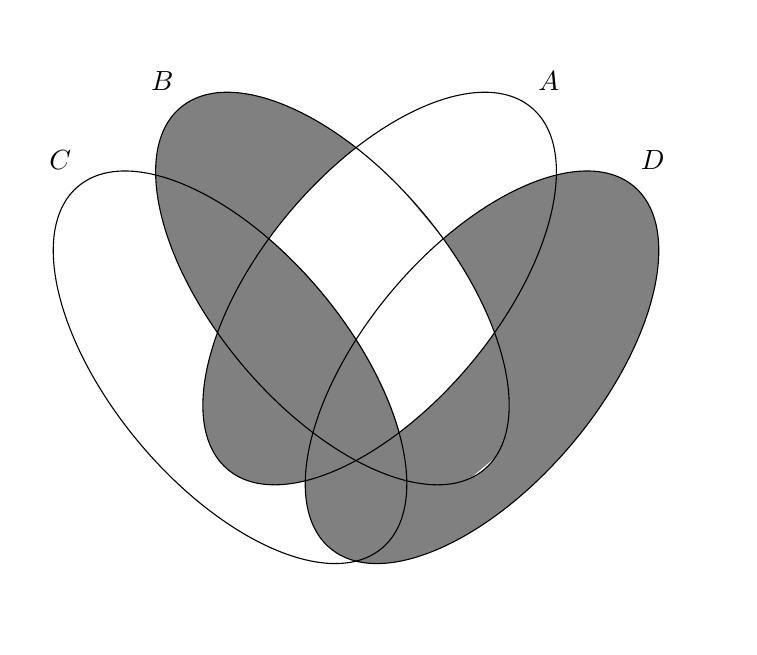
\begin{tikzpicture}

%definitions
\def\firstellip{(1.6, .4) ellipse [x radius=3cm, y radius=1.5cm,rotate=50]}
%
\def\secondellip{(0.3, 1.4cm) ellipse [x radius=3cm, y radius=1.5cm, rotate=50]}

\def\thirdellip{(-0.3, 1.4cm) ellipse [x radius=3cm, y radius=1.5cm, rotate=-50]}

\def\fourthellip{(-1.6, .4) ellipse [x radius=3cm, y radius=1.5cm, rotate=-50]}

\def\firstrect{[rotate around={50:(.85, -2.9)}](.85, -2.9) rectangle ++(6.05, 3.05)}

\def\secondrect{[rotate around={50:(-.45, -1.85)}](-.45, -1.85) rectangle ++(6.05, 3)}

\def\thirdrect{[rotate around={-50:(.45, -1.85)}](.45, -1.85) rectangle ++(-6.05, 3)}

\def\fourthrect{[rotate around={-50:(-.85, -2.9)}](-.85, -2.9) rectangle ++(-6.05, 3.05)}

\def\bounding{(-5,-3) rectangle (5,4)}

%fills

\begin{scope} %P1
\clip \secondellip;
\filldraw[gray] \fourthellip;
\end{scope}
%
\begin{scope}[even odd rule]
\clip \secondellip \thirdrect;
\fill[gray] \thirdellip;
\end{scope}

\begin{scope}[even odd rule]
\clip \thirdellip \firstrect;
\fill[gray] \firstellip;
\end{scope}

%shapes

\draw \firstellip node [outer sep=.8cm, above right, xshift=1.1cm, yshift=1.6cm] {$D$};

\draw \secondellip node [outer sep=.8cm, above right, xshift=1.1cm, yshift=1.6cm]{$A$};

\draw \thirdellip node [outer sep=.8cm, above left, xshift=-1.1cm, yshift=1.6cm]{$B$};

\draw \fourthellip node [outer sep=.8cm, above left, xshift=-1.1cm, yshift=1.6cm] {$C$};
\end{tikzpicture}

Conditionally valid. If you had a premise that told you to write an x in the $D$ ellipse, it would clearly fall outside of $C$.

\end{longtabu}


\begin{exercises}
\begin{longtabu}{X[1,p,m]X[1,p,m]}
\item \begin{kormanize}
\premise{No $D$ are $B$.
\premise{All $A$ are $C$.
\premise{All $C$ are $B$.
\conclusion{No $D$ are $A$.
\end{kormanize}

% Invalid
% * P --> A
% * M1 --> C
% * M2 --> B
% * S --> D

&
\item\begin{kormanize}
\premise{All $A$ are $B$.
\premise{No $D$ are $C$.
\premise{All $C$ are $A$. % All C are B
\conclusion{No $D$ are $B$.
\end{kormanize}

% Valid
% * P --> B
% * M1 --> A
% * M2 --> C
% * S --> D

\\
\item\begin{kormanize}
\premise{All $B$ are $D$. %Some $B$ are not $A$
\premise{All $B$ are $C$.
\premise{No $A$ are $D$.
\conclusion{Some $C$ are not $A$.
\end{kormanize}

% conditionally valid
% * P --> A
% * M1 --> D
% * M2 --> B
% * S --> C

&
\item\begin{kormanize}
\premise{No $A$ are $C$.
\premise{All $B$ are $D$.
\premise{All $C$ are $B$. %All C are D
\conclusion{No $A$ are $D$.
\end{kormanize}

% Valid, reduce terms
% * P --> D
% * M1 --> B
% * M2 --> C
% * S --> A

\\
\item\begin{kormanize}
\premise{All $D$ are $A$.
\premise{Some $C$ are $B$.
\premise{Some $B$ are not $D$.
\conclusion{Some non-$C$ are not non-$A$.
\end{kormanize}

% Invalid, reduce terms
% * P --> C
% * M1 --> B
% * M2 --> D
% * S --> A

&
\end{longtabu}
\end{exercises}

\noindent\problempart  Rewrite the following arguments in standard form, reducing terms if necessary, and then prove that they are valid using a single, four-term Venn diagram.

\begin{exercises}
\begin{longtabu}{X[1,p,m]X[1,p,m]}
\item \begin{kormanize}
\premise{No $A$ are $C$.
\premise{All $B$ are $D$.
\premise{Some $B$ are $A$.
\conclusion{Some $S$ are not $C$.
\end{kormanize}
%
%% Valid
%% * P --> C
%% * M1 --> A
%% * M2 --> B
%% * S --> D
%
&
\item\begin{kormanize}
\premise{No $P$ are $M$.
\premise{All $M$ are $M2$.
\premise{No $M2$ are $S$.
\conclusion{No $S$ are $P$.
\end{kormanize}
%
%% Invalid
%% * P --> B
%% * M1 --> A
%% * M2 --> C
%% * S --> D
%
\\
\item\begin{kormanize}
\premise{All $A$ are $C$.
\premise{All $B$ are $C$.
\premise{All $A$ are $D$.
\conclusion{Some $D$ are $B$.
\end{kormanize}

% Conditionally  valid
% * P --> B
% * M1 --> C
% * M2 --> A
% * S --> D

&
\item\begin{kormanize}
\premise{Some non-$D$ are not non-$C$.
\premise{All $D$ are $B$.
\premise{No $B$ are $A$.
\conclusion{Some $A$ are not $C$.
\end{kormanize}
% Invalid, reduce terms
% * P --> C
% * M1 --> D
% * M2 --> B
% * S --> A
\\
\item\begin{kormanize}
\premise{No $C$ are non-$B$.
\premise{Some $D$ are $A$.
\premise{All $D$ are $C$. %Some $C$ are $A$
\conclusion{Some $B$ are not $A$.
\end{kormanize}
% Valid, reduce terms
% * P --> A
% * M1 --> D
% * M2 --> C
% * S --> B

\end{longtabu}
\end{exercises}


\noindent\problempart Rewrite the following arguments in standard form using variables and a translation key. Then evaluate using any method you want. The example problem, along with exercises \ref{itm:sons}, \ref{itm:ducks},  \ref{itm:Auk}, and \ref{itm:rainbow}, come from Lewis Carroll's logic textbook \citep{Dodgson1896}. Other exercises are just Lewis Carroll themed.

\begin{longtabu}{p{.1\linewidth}p{.5\linewidth}p{.4\linewidth}}

\textbf{Example}: & \multicolumn{2}{p{.9\linewidth}}{My saucepans are the only things I have that are made of tin. I find all your presents very useful, but none of my saucepans are of the slightest use. Therefore, none of your presents are made of tin.} \\
\\
\textbf{Answer}:&
\vspace{-.5cm}
\begin{description}
\item[$A$:]Things of mine made from tin
\item[$B$:] Saucepans
\item[$C$:] Useful things
\item[$D$:] Presents from you
\end{description}

&
\vspace{-.5cm}
\begin{kormanize}
\premise{All $A$ are $B$.
\premise{No $B$ are $C$.
\premise{All $D$ are $C$.
\conclusion{No $D$ are $A$.
\end{kormanize}
\end{longtabu}
\vspace{-.75cm}
\begin{center}
\begin{tikzpicture}
\begin{scope}
% venns
\begin{scope}
\def\firstcircle{(0,0) circle (.75cm)}
\def\secondcircle{(60:.75cm) circle (.75cm)}
\def\thirdcircle{(0:.75cm) circle (.75cm)}

\begin{scope}
\clip \thirdcircle;
\fill[gray] \secondcircle;
\end{scope}

\begin{scope}[even odd rule] % Shade P without M
\clip \secondcircle (-1,-1) rectangle (2,2);
\fill[gray] \firstcircle;
\end{scope}

\draw \firstcircle node[outer sep=.66cm, below left] {$A$};
\draw \secondcircle node [outer sep=.75cm, above] {$B$};
\draw \thirdcircle node [outer sep=.66cm, below right] {$C$};

\end{scope}

\begin{scope}[xshift=4cm]

\def\firstcircle{(0,0) circle (.75cm)}
\def\secondcircle{(60:.75cm) circle (.75cm)}
\def\thirdcircle{(0:.75cm) circle (.75cm)}

\begin{scope} %shade overlap between S and M
\clip \thirdcircle;
\fill[gray] \secondcircle;
\end{scope}

\begin{scope}[even odd rule] % Shade P without M
\clip \secondcircle (-1,-1) rectangle (2,2);
\fill[gray] \firstcircle;
\end{scope}

\draw \secondcircle node [outer sep=.75cm, above] {$C$};
\draw \thirdcircle node [outer sep=.66cm, below right] {$A$};
\draw \firstcircle node[outer sep=.66cm, below left] {$D$};

\end{scope}

%% args

\node at (0,-2.5)[text width=4.5cm, outer sep=1mm] (Celarent){
\begin{kormanize}
\premise{All $A$ are $B$.
\premise{No $B$ are $C$.
\conclusion{No $A$ are $C$.*
\end{kormanize}

};

\node at (-.1, -3.9) {\textbf{Celarent (EAE-I)}};

\draw [myarrow1, ->] (1.1, -3.05) .. controls (2.4, -3) and (2.4, -2) .. (3.3, -1.95);
%
%\filldraw [red] (0,0) circle (.1cm);
%\filldraw [red] (2.4, -.5) circle (.1cm);
%\filldraw [red] (2.4, .5)  circle (.1cm);

\node at (5,-2.3)[text width=4.5cm, outer sep=1mm] {
\begin{kormanize}
\premise{No $A$ are $C$.*
\premise{All $D$ are $C$.
\conclusion{No $D$ are $A$.
\end{kormanize}
%Cesare (EAE-II)
};

\node at (4.9, -3.9) {\textbf{Cesare (EAE-II)}};
\end{scope}
\end{tikzpicture}
\end{center}

\begin{exercises}

\item All metal things are solid, and some of those metal things are also chairs. All chairs are furniture. Therefore some solid things are furniture.

%Three premise valid


%\begin{kormanize}
%\premise{All $M1$ are $P$
%\premise{Some $M2$ are $M1$
%\premise{All $M2$ are $S$
%\vspace{-.5em}
% \item [] \rule{0.6\linewidth}{.5pt}
%\item[C:] Some $S$ are $P$
% \end{kormanize}


\item \label{itm:sons} Every one who is sane can do Logic. No lunatics are fit to serve on a jury. None of \textit{your} sons can do Logic. Therefore, none of your sons can serve on a jury.

%three premise valid

\item All hat-wearers are heaven-sent. This is because all platypuses are heaven-sent, all secret agents are platypuses, and some secret agents wear hats.

%\begin{kormanize}
%\premise{All platypuses are heaven-sent
%\premise{All secret agents are platypuses     %All $C$ are $A$
%\premise{Some secret agents wear hats
%\vspace{-.5em}
% \item [] \rule{0.6\linewidth}{.5pt}
%\item[C:] All hat-wearers are heaven-sent
% \end{kormanize}


\item \label{itm:ducks} No ducks waltz. No officers ever decline to waltz. All my poultry are ducks. Therefore, none of my poultry are officers.



%\begin{kormanize}
%\premise{All my poultry are ducks
%\premise{No ducks waltz
%\premise{All officers waltz
%\vspace{-.5em}
%\item [] \rule{0.6\linewidth}{.5pt}
%\item[C:] None of my poultry are officers
%\end{kormanize}

\item Some things are uffish, but nothing that is uffish is vorpal. Therefore some uffish things are not swords, because everything that is vorpal goes snicker-snack, and everything that goes snicker-snack is a sword.

%\begin{description}
%\item[$A$:] Swords.
%\item[$B$:] Things that go snicker-snack
%\item[$C$:] Vorpal things.
%\item[$D$:] Uffish things
%\end{description}



%\begin{kormanize}
%\premise{Everything that goes snicker-snack is a sword.
%\premise{Everything that is vorpal goes snicker-snack
%& Everything that is vorpal is a sword
%\premise{Nothing uffish is vorpal
%\item[{\color{red}P$_4$:}] {\color{red}Some uffish things exist.}
%\vspace{-.5em}
%\item [] \rule{0.2\linewidth}{.5pt}
%\item[C:] Some uffish things are not swords
%\end{kormanize}

%\begin{kormanize}
%\premise{All $B$ are $A$.
%\premise{All $C$ are $B$
%\premise{No $D$ are $C$
%\item[{\color{red}P$_4$:}] {\color{red}$D$ exists.}
%\vspace{-.5em}
%\item [] \rule{0.2\linewidth}{.5pt}
%\item[C:] Some $D$ are not $A$
%\end{kormanize}

\item No animals are plants. Some animals are mammals. Some mammals are dogs. All dachshunds are dogs. Therefore, no dachshunds are plants.


%\begin{kormanize}
%\premise{No $B$ are $A$
%\premise{Some $B$ are $C$.    % Therefore, some $C$ are not $A$.
%\premise{Some $C$ are $D$
%\premise{All $E$ are $D$
%\vspace{-.5em}
%\item [] \rule{0.6\linewidth}{.5pt}
%\item[C:]  No $E$ are $A$.
%\end{kormanize}


\item \label{itm:Auk} Things sold in the street are of no great value. Nothing but rubbish can be had for a song. Eggs of the Great Auk are very valuable. It is only what is sold in the streets that is really rubbish. Therefore the eggs of the Great Auk cannot be had for a song.

%\begin{kormanize}
%\premise{Nothing but rubbish can be had for a song
%\premise{It is only what is sold in the streets that is really rubbish.
%\premise{Things sold in the street are of no great value;
%\premise{Eggs of the Great Auk are very valuable
%\vspace{-.5em}
%\item [] \rule{0.6\linewidth}{.5pt}
%\item[C:] The eggs of the Great Auk cannot be had for a song
%\end{kormanize}

%\begin{description}
%\item[$A$:] Things you can have for a song
%\item[$B$:] Rubbish
%\item[$C$:] Valuable things
%\item[$D$:] Things sold in the street
%\item[$E$:] Eggs of the Great Auk
%\end{description}

%\begin{kormanize}
%\premise{All $A$ are $B$
%\premise{All $B$ are $C$
%\premise{No $C$ are $D$;
%\premise{All $E$ are $D$
%\vspace{-.5em}
%\item [] \rule{0.6\linewidth}{.5pt}
%\item[C:] No E are A.
%\end{kormanize}

\item All life forms are physical objects, and all bacteria are life forms. Also, all \textit{E. coli} are bacteria, so all rod shaped things are physical objects, because all \textit{E. coli} are rod-shaped.

% four premise invalid

%\begin{kormanize}
%\premise{All $B$ are $A$
%\premise{All $C$ are $B$
%\premise{All $D$ are $C$;
%\premise{All $D$ are $E$
%\vspace{-.5em}
%\item [] \rule{0.6\linewidth}{.5pt}
%\item[C:] All E are A.
%\end{kormanize}




\item Some playing cards shout ``Off with his head!'' All playing cards play croquet. Everyone who plays croquet uses hedgehogs for balls. Everyone who uses hedgehogs for balls uses flamingos for mallets. The queen of hearts uses flamingos for mallets. Therefore some cards identical to the queen of hearts shout ``Off with his head!''

%Playing cards
%``shout off with his head'!'
%Plays croquet
%Uses hedgehogs for balls
%uses flamingos for mallets
%Is identical to the queen of hearts

%\begin{kormanize}
%\premise{Some $B$ are $A$
%\premise{All $B$ are $C$     %Some $C$ are $A$ 	Disamis (IAI-III) (valid)
% \premise{All $C$ are $D$ 	% Some $D$ are $A$ %		Disamis (IAI-III) (valid)
%\premise{All $D$ are $E$ % Some $E$ are $A$ Disamis (IAI-III) (valid)
%\item[P$_5$:] All $F$ are $E$
% \item [] \rule{0.6\linewidth}{.5pt}
%\item[C:] Some $F$ are $A$ % IAI-I (invalid)
% \end{kormanize}

%\begin{kormanize}
%\premise{Some $B$ are $A$
%\premise{All $B$ are $C$
%\vspace{-.5em}
% \item [] \rule{0.6\linewidth}{.5pt}
%\item[IC$_1$:] Some $C$ are $A$
% \end{kormanize} Disamis (IAI-III) (valid)

%\begin{kormanize}
%\item[IC$_1$:] Some $C$ are $A$
%\premise{All $C$ are $D$
%\vspace{-.5em}
% \item [] \rule{0.6\linewidth}{.5pt}
%\item[IC$_2$:] Some $D$ are $A$
% \end{kormanize} Disamis (IAI-III) (valid)

%\begin{kormanize}
%\item[IC$_2$:] Some $D$ are $A$
%\premise{All $D$ are $E$
%\vspace{-.5em}
% \item [] \rule{0.6\linewidth}{.5pt}
%\item[IC$_3$:] Some $E$ are $A$
% \end{kormanize} Disamis (IAI-III) (valid)

%\begin{kormanize}
%\item[IC$_3$:] Some $E$ are $A$
%\item[P$_5$:] All $F$ are $E$
% \item [] \rule{0.6\linewidth}{.5pt}
%\item[C:] Some $F$ are $A$
% \end{kormanize} IAI-I (invalid)



\item \label{itm:rainbow} I despise anything that cannot be used as a bridge. Everything, that is worth writing an ode to, would be a welcome gift to me. A rainbow will not bear the weight of a wheelbarrow.  Whatever can be used as a bridge will bear the weight of a wheel-barrow. I would not take, as a gift, a thing that I despise. Therefore a rainbow is not worth writing an ode to.

%\begin{kormanize}
%\premise{Everything, that is worth writing an ode to, would be a welcome gift to me
%\premise{I would not take, as a gift, a thing that I despise.
%\premise{I despise anything that cannot be used as a bridge;
%\premise{Whatever can be used as a bridge will bear the weight of a wheel-barrow;
%\item[P$_5$:] A rainbow will not bear the weight of a wheelbarrow;
%\vspace{-.5em}
%\item [] \rule{0.6\linewidth}{.5pt}
%\item[C:] A rainbow is not worth writing an ode to.
%\end{kormanize}
\end{exercises}

\noindent\problempart Rewrite the following arguments in standard form using variables and a translation key, and supply intermediate conclusions. Then evaluate using any method you want. Exercises \ref{itm:talkers}, \ref{itm:hedgehogs}, \ref{itm:mermaids}, \ref{itm:books}, and \ref{itm: poems} come from Lewis Carroll's logic textbook \citep{Dodgson1896}. Other exercises are just Lewis Carroll themed.

\begin{exercises}

\item All buildings are habitable places, and all houses are residences. Therefore all houses are buildings because all residences are habitable places.

%\begin{kormanize}
%\premise{All $A$ are $B$
%\premise{All $C$ are $B$		%All $C$ are $A$
%\premise{All $D$ are $C$
%\vspace{-.5em}
%\item [] \rule{0.6\linewidth}{.5pt}
%\item[C:]  All $D$ are $A$
%\end{kormanize}


\item Not all cephalopods are moralizing, but cuttlefish are. All pompous squid are cephalopods. Therefore some pompous squid are not cuttlefish.

%
%\begin{kormanize}
%\premise{All $A$ are $B$
%\premise{Some $C$ are not $B$		%Some $C$ are not $A$
%\premise{All $D$ are $C$
%\vspace{-.5em}
%\item [] \rule{0.6\linewidth}{.5pt}
%\item[C:] Some $D$ are not $A$
%\end{kormanize}

%AEE-II, EAO-1


\item \label{itm:talkers} Showy talkers think too much of themselves; No really well-informed people are bad company; and people who think too much of themselves are not good company. Therefore no showy talkers are really well informed. %[three premise] LC


%\begin{kormanize}
%\premise{No really well-informed people are bad company;
%\premise{People who think too much of themselves are not good company.
%\premise{Showy talkers think too much of themselves;
%\vspace{-.5em}
%\item [] \rule{0.6\linewidth}{.5pt}
%\item[C:] No one who thinks too much of themselves is really well informed.
%\end{kormanize}

%\begin{description}
%\item[$A$:] Well informed people.
%\item[$B$:] Good company
%\item[$C$:] People who think too much of themselves.
%\item[$D$:] Showy talkers
%\end{description}

%\begin{kormanize}
%\premise{All $A$ are $B$    %No $A$ are non-$B$
%\premise{No $C$ are $B$.    %No $C$ are $A$ camestres
%\premise{All $C$ are $D$;
%\vspace{-.5em}
%\item [] \rule{0.6\linewidth}{.5pt}
%\item[C:] No $D$ are $A$
%\end{kormanize}



\item All white animals are late, and some late animals are rabbits. Also, all animals taking a watch out of their waistcoat pocket are white. Therefore, some rabbits are taking a watch out of their waistcoat pocket.


%$A$: animals taking a watch out of their waistcoat pocket.
%B: White animals
%C: Late animals
%D: Rabbits


%\begin{kormanize}
%\premise{All animals taking a watch out of their waist-coat pocket are white
%\premise{All white animals are late 			All $M2$ are $P$
%\premise{Some late animals are rabbits
%\vspace{-.5em}
%\item [] \rule{0.6\linewidth}{.5pt}
%\item[C:] Some rabbits are taking a watch out of their waist-coat pocket.
%\end{kormanize}


%\begin{kormanize}
%\premise{All A are B
%\premise{All B are C 			All A$ are C
%\premise{Some C are D
%\vspace{-.5em}
%\item [] \rule{0.6\linewidth}{.5pt}
%\item[C:] Some D are A.
%\end{kormanize}

\item \label{itm:hedgehogs} No one takes in the \textit{Times} unless he is well-educated. But no hedge-hogs can read, and those who cannot read are not well-educated. Therefore no hedge-hog takes in the \textit{Times}.

\item The Red Queen is a chess piece. Among the things that have to run faster and faster just to stay in the same place is the Red Queen. All lost children have to run faster and faster just to stay in the same place. Alice is a lost child. Therefore, Alice is one of the chess pieces.

%\begin{kormanize}
%\premise{All $B$ are $A$
%\premise{Some $C$ are $B$  %Some $C$ are $A$  Darii (AII-1) (valid)
%\premise{All $D$ are $C$
%\premise{All $E$ are $D$
%\vspace{-.5em}
% \item [] \rule{0.6\linewidth}{.5pt}
%\item[C:] Some $E$ are $A$
% \end{kormanize}

\item \label{itm:mermaids} None of the unnoticed things met with at sea are mermaids. Things entered in the log as met with at sea are sure to be worth remembering. I have never met with anything worth remembering, when on a voyage. Things met with at sea, that are noticed, are sure to be recorded in the log. Therefore, I have never come across a mermaid at sea. %[four premise] LC


%\begin{description}
%\item[$A$:] Mermaids
%\item[$B$:] Things noticed
%\item[$C$:] Things recorded in the log
%\item[$D$:] Things worth remembering.
%\item[$E$:] Things met by me.
%\end{description}



%\begin{kormanize}
%\premise{All $A$ are $B$   %Starts are ``No $A$ are non-$B$''
%\premise{All $A$ are $C$
%\premise{All $C$ are $D$
%\premise{No $E$ are $D$
%\vspace{-.5em}
%\item [] \rule{0.6\linewidth}{.5pt}
%\item[C:] No $E$ are $A$
%\end{kormanize}

\item \label{itm:plum-pudding} A plum-pudding that is not really solid is mere porridge. Every plum-pudding served at my table has been boiled in a cloth. A plum-pudding that is mere porridge is indistinguishable from soup. No plum puddings are really solid except what are served at my table. Therefore no plum-pudding that has not been boiled in cloth can be distinguished from soup. %[four premise] LC

\item \label{itm:books} The only books in this library that I do \textit{not} recommend for reading are unhealthy in tone. All the bound books are well-written. All the romances are healthy in tone, and I do not recommend you read any of the unbound books. Therefore all the romances in this library are well-written.

\item \label{itm: poems} No interesting poems are unpopular among people of real taste. No modern poetry is free from affectation. All \textit{your} poems are on the subject of soap bubbles. No affected poetry is popular among people of real taste. No ancient poem is on the subject of soap-bubbles. Therefore all of \textit{your} poems are uninteresting. %[five premise] LC

\end{exercises}

\noindent\problempart
\begin{exercises}
\item Suppose you wanted to represent five terms using a Venn diagram. How would you arrange the ellipses?
\item Can you figure out a principle for continually adding shapes to a Venn diagram that will always allow you to represent every combination of terms?
\end{exercises}

%
% Below is the closing tag for typesetting only part of the chapter. Everything up to here to the close tag will be skipped unless the {whole_syl_chap} label at the start of this chapter file is
%  uncommented.

}{}
